\documentclass[10pt]{report}
\usepackage{/Users/bradenhoagland/latex/math}

\lhead{Braden Hoagland}
\chead{Real Analysis}
\rhead{}

\begin{document}

\tableofcontents

\chapter{The Real Line and Euclidean Space}

\section{Ordered Fields and the Number Systems}

\begin{defn}{Ordered Field}{ordered-field}
	An ordered field is a field equipped with a subset $R \subset F \times F$ s.t. $x \leq y$ if $(x,y)  \in \mathbb{R}$.
\end{defn}

$R$ must satisfy
\begin{enumerate}
	\item $x \leq x$
	\item $x \leq y, y \leq x \implies x = y$ 
	\item $x \leq y, y \leq z \implies x \leq z$
	\item $x, y \in F \implies x \leq y$ or $y \leq x$
	\item $x \leq y \implies x + z \leq y + z$
	\item  $0 \leq x, 0 \leq y \implies 0 \leq xy$
\end{enumerate}

For ordered fields, $x^2 \geq 0$.

\begin{prop}
	Let F be an ordered field, then for $x,y \in F$ 
\end{prop}
\begin{enumerate}
	\item $|x+y| \leq |x| + |y|$
	\item $\big| |x| - |y| \big| \leq |x-y|$
	\item $|xy| \leq |x||y|$
\end{enumerate}

\begin{defn}{Principle of Mathematical Induction}{induction}
	If $S \in \mathbb{N}$ s.t. $1 \in S$ and $k \in S \implies k+1 \in S$, then $S = \mathbb{N}$.
\end{defn}

\begin{defn}{Well Ordering Principle}{well-ordering}
	If $S \in \mathbb{N}$ s.t. $S \neq \{0\}$, then there exists $\sigma \in S$ s.t. $\sigma \leq n$ for all $n \in S$ (a smallest element exists).
\end{defn}

\begin{ex}{}{}
$\mathbb{N}$ is well-ordered, but $ \mathbb{Z}$ is not.
\end{ex}

\begin{defn}{Countable}{}
	A set $S$ is \textbf{countable} if there is an injection $f : S \xhookrightarrow{} \mathbb{N}$
\end{defn}

\begin{prop}
	$ \mathbb{N} \times \mathbb{N}$ is countable.
\end{prop}
\begin{proof}
	Set $f(m,n) = 2^m (2n-1)$. This is injective.
\end{proof}

\begin{cor}
	If $X$ and $Y$ are countable, $X \times Y$ is countable.
\end{cor}
\begin{proof}
	We know there exist $\phi: X \xhookrightarrow{} \mathbb{N}$ and $\psi: Y  \xhookrightarrow{} \mathbb{N}$. Form the map $(\phi, \psi) : X \times Y \xhookrightarrow{} \mathbb{N} \times \mathbb{N}$, then $f \circ (\phi, \psi)  \xhookrightarrow{} \mathbb{N}$	
\end{proof}

\begin{cor}
	$\mathbb{Z}$ is countable.
\end{cor}
\begin{proof}
	Let $g: \mathbb{Z} \to \mathbb{N}_0 \times \mathbb{N}_0$ be defined by $g(m) = (m,0)$ if $m \geq 0$ and $g(m) = (0, -m)$ if $m < 0$. Since $\mathbb{N}_0$ is countable ($m \mapsto m+1)$, we know $\mathbb{N}_0 \times \mathbb{N}_0$ is countable, and thus $\mathbb{Z}$ is also countable.
\end{proof}

\begin{cor}
	$\mathbb{Q}$ is countable.
\end{cor}
\begin{proof}
	Let $p/q \in \mathbb{Q}$ with $q > 0$ and $p,q$ relatively prime. Define $g : \mathbb{Q} \xhookrightarrow{} \mathbb{Z} \times \mathbb{N}$ by $g(p/q) = (p,q)$. Since $\mathbb{Z} \times \mathbb{N}$ is countable, so is $\mathbb{Q}$.
\end{proof}

\begin{prop}
	$\mathbb{Q}$ is dense in itself: If $x,y \in \mathbb{Q}$, then there is a $z \in \mathbb{Q}$ such that $x < z < y$.
\end{prop}
\begin{proof}
	Let $z = (x+y)/2$. This works.
\end{proof}

\begin{defn}{Archimedean Property}{arch}
	If $x \in \mathbb{Q}$, then there exists  $n \in \mathbb{N}$ such that $x < n$.
\end{defn}
\begin{proof}
	If $x < 0$, take $n=1$. If $x = p/q$ with $p,q > 0$, take $n = p+1$. This works because
	\[
		\frac{p}{q} \leq \frac{p}{q} + (q-1) \frac{p}{q} = p < p+1
	\] 
\end{proof}

\begin{defn}{Field Isomorphism}{field-iso}
	Let $S_1$ and $S_2$ be two fields. A bijective function $\phi: S_1 \leftrightarrow S_2$ is a field isomorphism if $\phi(x+y) = \phi(x)+\phi(y)$ and $\phi(xy) = \phi(x) \phi(y)$. If such a $ \phi$ exists, we say that $S_1$ and $S_2$ are isomorphic.
	Additionally, if $S_1$ and $S_2$ are ordered fields and $x \leq y \implies \phi(x) \leq \phi(y)$, then $\phi$ is called an ordered field isomorphism.
\end{defn}

\begin{prop}
	If $F$ is an ordered field, then there exists  $\mathbb{Z}_F \subset F$ such that $\mathbb{Z}_F$ (with inherited arithmetic) is ring isomorphic to $\mathbb{Z}$.
\end{prop}
\begin{proof}
	$0_F, 1_F, -1_F \in F$. By the properties of fields, 
	\begin{align*}
		0_F &< 1_F \\
		1_F &< 1_F + 1_F \\
		    &\vdots
	\end{align*}
	Define $\phi: \mathbb{N} \leftrightarrow F$ by $\phi(n) = \underbrace{1_F + \cdots + 1_F}_{n \text{ times}}$ and $\phi(-n) = -\phi(n)$.
\end{proof}

\begin{prop}
	Similarly, there exists $\mathbb{Q}_F \in F$ such that $\mathbb{Q}_F$ is an ordered field $\simeq \mathbb{Q}$.
\end{prop}

\begin{defn}{Archimedean Ordered Field}{arch-ord-field}
	An ordered field $F$ is Archimedean if for all $x \in F$, there exists $n \in \mathbb{N}_F$ such that $x<n$.
\end{defn}

\begin{prop}
	The following are equivalent to the original definition of an Archimedean ordered field.
	\begin{enumerate}
		\item $0<y<x \implies$ there exists $k \in \mathbb{N}$ such that $x < ky$.
		\item $x > 0 \implies$ there exists $n \in \mathbb{N}$ such that $0 < \frac{1}{n} < x$.
	\end{enumerate}
\end{prop}
\begin{proof}
	\begin{enumerate}
		\item Assume $F$ is Archimedean, then $x y^{-1}<k$ for some $k \in \mathbb{N}$, which implies $x < ky$. Conversely, if (1) holds, then we have two cases. If $x \leq 1$, then it is clearly bounded above by, say, 2. If $1 < x$, then take $y=1$, then there exists $k$ such that $x < k$.
		\item The proof for the second formulation is similar.
	\end{enumerate}
\end{proof}

\section{Completeness and the Real Number System}

$\mathbb{Q}$ satisfies all the properties of an ordered field, so we need something more to characterize $\mathbb{R}$. This will be ``completeness", where the limits of rationals are in the system too. This requires the use of sequences and limits.

\begin{defn}{Sequence}{seq}
	A function $f:\mathbb{N} \to S$, where $S$ is a set, is a sequence in $S$. We often denote $f(n)$ by $a_n$ and $f$ by $\{a_n\}_{n=1}^\infty$.
\end{defn}

\begin{defn}{Subsequence}{subseq}
	Let $f:\mathbb{N}\to S$ be a sequence. Let $ \sigma:\mathbb{N} \hookrightarrow \mathbb{N}$ be injective and increasing, i.e. $\sigma(n+1) > \sigma(n)$. Then $f \circ \sigma$ is called a \textbf{subsequence} of $f$.
\end{defn}

Useful notation for subsequences is $\left\{ x_{\sigma(n)} \right\}_{n=1}^\infty$ instead of $\left\{ x_{n} \right\}_{n=1}^\infty$.

\begin{defn}{Convergence}{conv-ord-field}
	A sequence $\{a_n\}_{n=1}^\infty$ in an ordered field $F$ converges to a limit $L$ if for all $\varepsilon > 0$ in $F$, there exists $N \in \mathbb{N}$ such that $|a_n - L| < \varepsilon$ if $n > N$.
\end{defn}

Intuitively, this means that all but finitely many $a_n$ lie outside of the interval $(L-\varepsilon, L+\varepsilon)$.

\begin{prop}{Squeeze Lemma}
	If $x_n \to L$ and $z_n \to L$ and $x_n \leq y_n \leq z_n$ for any $n > n_0$, then $y_n \to L$.
\end{prop}
\begin{proof}
Since $x_n$ and $z_n$ converge to $L$, for any $\varepsilon>0$ there exist $N_x$ such that $|x_n-L| < \varepsilon$ when $n > N_x$ and $N_z$ such that $|z_n-L|<\varepsilon$ when $n > N_z$.

Let $N = \max\left\{ n_0, n_x, n_z \right\}$, then we have
\[
-\varepsilon < x_n - L \leq y_n - L \leq z_n - L < \varepsilon.
\] Thus $y_n \to L$.
\end{proof}

Similarly, if $a \leq x_n \leq b$ and $x_n \to L$, then $a \leq L \leq b$.

\begin{prop}
	In an Archimedean field, if $x_n \to x$ and $x_n \to y$, then $x=y$, i.e. limits are unique.
\end{prop}
\begin{proof}
	By the triangle inequality, we have
	\[
	|x-y| = |x-x_n+x_n-y| \leq |x-x_n|+|x_n-y|.
	\] 
	Suppose $|x-y| > 0$, then set $\varepsilon = |x-y|/2$. We can then choose $N$ large enough that
	\[
	|x-y|\leq |x-x_n|+|x_n-y| < \frac{|x-y|}{2} + \frac{|x-y|}{2} = |x-y|.
	\] 
	This is a contradiction, so $|x-y| = 0$.
\end{proof}

\subsection{Bounded Sequences}

\begin{defn}{Bounded}{bounded-arch-field}
	Let $F$ be an Archimedean field, then $S \subset F$ is bounded if there exists $M \in F$ such that $|\sigma| \leq M$ for all $\sigma \in S$.
\end{defn}
A function can be also just bounded below or above, which is a weaker condition.

\begin{prop}
	A convergent sequence in an Archimedean field is bounded.
\end{prop}
\begin{proof}
	Suppose $x_n \to L$, then there exists $N$ such that $|x_n-L| < 1$ if  $n > N$ (the choice of $1$ here is arbitrary). Then for $n > N$,
	\[
	|x_n| = |x_n - L + L| \leq |x_n-L| + |L| < 1 + |L|
	\]
	Set the bound $M = \max\{|x_1|, |x_2|, \dots, |x_n|, 1 + |L|\}$.
\end{proof}

\subsection{Limit Arithmetic}

\begin{prop}
Some of the usual arithmetic operations also hold with limits. Let $x_n \to x$ and $y_n \to y$, then
\begin{enumerate}
	\item $x_n + y_n \to x+y$
	\item $\lambda x_n \to \lambda x$
	\item $x_n y_n \to xy$ 
	\item $y_n \neq 0, y \neq 0 \implies x_n y_n^{-1} \to xy^{-1}$
\end{enumerate}
\end{prop}
\begin{proof}
	Each of these proofs is based on simple applications of the triangle inequality.
	\begin{enumerate}
		\item Since $x_n \to x$ and $y_n \to y$, for all $\varepsilon>0$, there exist $N_x$ such that $|x-x_n| < \varepsilon/2$ when $n > N_x$ and $N_y$ such that $|y-y_n|<\varepsilon/2$ when $n>N_y$. Let $N = \max{N_x,N_y}$, then for all $\varepsilon>0$,
			\[
				|(x_n+y_n) - (x+y)| \leq |x_n - x| + |y_n - y| < \varepsilon.
			\] 

		\item This is a special case of $(3)$, so it suffices to prove $(3)$.

		\item We have
			\[
			|x_n y_n - xy| = |x_n y_n - x_n y + x_n y - xy| \leq |x_n| |y_n-y| + |y||x_n-x|.
			\] 
			Since $\left\{ x_n \right\}$ converges, it is bounded, i.e. $|x_n| \leq M$ for all $n$. Let $\tilde{M} = \max\{M, |y|\}$. Then our inequality becomes
			\[
			|x_n y_n - xy| \leq \tilde{M}|y_n-y| + \tilde{M} |x_n-x|.
			\] 
			For $\varepsilon>0$, choose $N$ such that $|x_n-x|, |y_n-y| < \varepsilon/(2\tilde{M})$ for all $n > N$, then $|x_n y_n - xy| < \varepsilon$.

		\item Since $y_n,y\neq_0$, we have
			\begin{align*}
				| x_n y_n^{-1}-xy^{-1}| &= \left| \frac{x_n y - x y_n}{y_n y} \right| \\
							&= \left| \frac{x_n y - xy + xy - x y_n}{y_n y} \right| \\
							&\leq \frac{|y| |x_n-x|}{|y_n y|} + \frac{|x| |y-y_n|}{|y_ny|} \\
							&\leq |y|^2 |y_n| |x_n-x| + |x||y||y_n||y-y_n|
			\end{align*}
			Since $\left\{ y_n \right\}$ converges, it is bounded, i.e. $|y_n| \leq M_y$ for all $n$. Let $M = \max\{|x|,|y|\} \cdot M_y$. Then for any $\varepsilon>0$, we can find $N$ large enough such that $|x_n-x|,|y_n-y| < \varepsilon/(2M)$. This yields
			\[
			| x_n y_n^{-1}-xy^{-1}| \leq M |x_n-x| + M |y_n-y| < \varepsilon.
			\] 
	\end{enumerate}
\end{proof}

\subsection{Completeness}

The terms ``nondecreasing", ``nonincreasing", ``strictly decreasing", and ``strictly increasing" all describe monotone sequences.

\begin{defn}{Monotone Sequence Property}{MSP}
	Let $F$ be an ordered field. We say that $F$ has the Monotone Sequence Property if every monotone increasing sequence bounded above converges.
\end{defn}

\begin{defn}{Completeness}{complete-ord-field}
	An ordered field is complete if it obeys the Monotone Sequence Property.
\end{defn}

Complete ordered fields are Archimedean.

\subsection{The Real Numbers}

\begin{thrm}{The Real Number System}{real-numbers}
	There's a unique (up to isomorphism) complete ordered field called the real number system. It is constructed as follows:
	Let $S$ be defined
	\[
		S = \left\{ (x_1, x_2, \dots) | x_n \in \mathbb{Q} \text{, sequence is increasing and bounded above} \right\}
	\] 
	and let two members of $S$ be equivalent if their upper bounds are the same. Then $\mathbb{R}$ is the set of all equivalence classes in $S$. We do not include $\pm \infty$ in $\mathbb{R}$.
\end{thrm}

\begin{prop}
$\mathbb{Q}$ is dense in $\mathbb{R}$. This can be stated two ways:
\begin{enumerate}
	\item $x,y \in \mathbb{R}$ with $x<y$, then there exists $r \in \mathbb{Q}$ with $x < r < y$
	\item If  $x,\varepsilon \in \mathbb{R}$ with $\varepsilon > 0$, then there exists $r \in \mathbb{Q}$ with $|x-r| < \varepsilon$.
\end{enumerate}
\end{prop}
\begin{proof}
	Suppose $x<y$, so $y-x>0$. Then since $\mathbb{R}$ is Archimedean, there exists an integer $n$ such that $0 < 1/n < y-x$, as well as another integer $k$ such that $k/n > x$. By the well-ordering property, there is a smallest such $k$. Using this smallest $k$, we have $(k-1)/n \leq x < k/n$. Let $r=k/n$ (which is clearly rational), then
	\[
		x < r = \frac{k-1}{n} +\frac{1}{n} \leq x + \frac{1}{n} < x + (y-x) = y.
	\] 
	So $x<r<y$, as required.
\end{proof}

Although $\mathbb{Q}$ is dense in $\mathbb{R}$, there are actually many more irrationals than rationals.

\begin{thrm}{}{reals-uncountable}
	The interval $(0,1)$ in $\mathbb{R}$ is uncountable.
\end{thrm}

Since the function $f(x) = a + (b-a)x$ maps $]0,1[ \mapsto ]a,b[$, any interval in $\mathbb{R}$ is uncountable. Since $\mathbb{R}$ is uncountable but $\mathbb{Q}$ is countable, it must be the case that $\mathbb{C}$ is uncountable.

\section{Infimums and Supremums}

\begin{defn}{Least Upper Bound/Supremum}{sup}
	Let $S \subset \mathbb{R}$, then $b$ is an \textbf{upper bound} for $S$ if for all $x \in S$, $x \leq b$. Additionally, $b$ is a \textbf{least upper bound}  of $B$ if
	\begin{enumerate}
		\item $b$ is an upper bound of $S$ 
		\item $b \leq u$ for every other upper bound $m$ of $S$
	\end{enumerate}
	If $S \subset \mathbb{R}$ is not bounded above or is empty, then $ \sup S = \infty$.
\end{defn}

Least upper bounds are unique. If $b$ is an upper bound of $S$ and $b \in S$, then $b$ is the least upper bound.

\begin{prop}
	Let $S \subset \mathbb{R}$ be nonempty. Then $b \in \mathbb{R}$ is the least upper bound of $B$ if and only if $b$ is an upper bound of $S$ and for every $\varepsilon > 0$ there is an $x \in S$ such that $x > b-\varepsilon$.
\end{prop}
\begin{proof}
	\textbf{Forward:} By definition, a least upper bound is an upper bound. Let $\varepsilon>0$, then $b-\varepsilon/2<b$ is not an upper bound. Then there exists some $x\in S$ such that if $b-\varepsilon/2\leq x$, then $x>b-\varepsilon$.

	\textbf{Backward:} Let $y<b$ and set $\varepsilon=b-y$. Since $y=b-\varepsilon$, there exists $x\in S$ such that $y<x$. Then  $y$ is not a least upper bound. This implies that $b$ is the least upper bound.
\end{proof}

\begin{defn}{Greatest Lower Bound/Infimum}{inf}
	You can guess the definition of this from how the supremum was defined. If the set $S$ is unbounded of empty, $\inf S = -\infty$.
\end{defn}

\begin{prop}
	Let $A \subset B \subset \mathbb{R}$, then $\inf B \leq \inf A \leq \sup A \leq \sup B$.
\end{prop}
\begin{proof}
	$\inf B \leq b$ for any $b \in B$, but any element $a \in A$ is also in $B$, so $\inf B \leq a$ for any $a \in A$. Thus $\inf B \leq \inf A$. Similarly, $\sup B \geq b$ for all $b \in B$, but since $a \in A \implies a \in B$, $\sup B \geq a$ for all $a \in A$. The middle inequality is trivial.
\end{proof}

\begin{thrm}{}{}
	In $\mathbb{R}$ the following hold
	\begin{enumerate}
		\item Least upper bound property: Let $S \subset \mathbb{R}$ be non-empty and have an upper bound, then $S$ also has a least upper bound.
		\item Greatest lower bound property: Let $S \subset \mathbb{R}$ be non-empty and have a lower bound, then $S$ also has a greatest lower bound.
	\end{enumerate}
\end{thrm}
\begin{proof}
	We only prove the first half of this theorem. The second half holds by symmetry.

	We can construct a decreasing sequence bounded below by the value that ends up being our least upper bound. Let $M$ be an upper bound of $S$, and let $n$ be a positive integer. Consider the sequence $M-1/2^n, M-2/2^n, M-3/2^n, dots$ that steps down by $1/2$ at every point. Choose the first integer $k$ such that $M - k/2^n$ fails to be an upper bound, and denote this by $k_n$ (such a $k_n$ is guaranteed to exist since $S$ is nonempty and $\mathbb{R}$ is Archimedean).

	Let $b_n = M - k_n/2^n$, so that $b_n$ is \textit{not} an upper bound but $b_n + 1/2^n$ \textit{is} an upper bound. Since a larger $k$ results in smaller steps, it is clear that $\left\{ b_i \right\}$ is an increasing sequence bounded above by $M$. Then by the completeness of $\mathbb{R}$, $b_n \to b$ for some $b$, which we claim to be the least upper bound. Note that $b_n \leq b$ for all $n$.

	To see this, assume $x \in S$ is greater than $b$. Then $x - b = \varepsilon$ for some $\varepsilon>0$. Choose $n$ large enough that $1/2^n < \varepsilon$, then
	\[
	x = b + \varepsilon \geq b_n +\varepsilon > b_n + 1/2^n.
	\] 
	By construction, this is impossible. So by contradiction, there can be no elements of $S$ that are larger than $b$. Thus $b$ is the least upper bound of $S$.
\end{proof}
This theorem is equivalent to the completeness axiom for an ordered field.

\section{Cauchy Sequences}

\begin{defn}{Cauchy Sequence}{cauchy-real}
	A sequence $x_n$ of real numbers is a Cauchy sequence if for all $\varepsilon>0$, there is an integer $N$ such that $|x_n-x_m|<\varepsilon$ whenever $n >N$ and $m>N$.
\end{defn}

\begin{prop}
	Every convergent sequence is a Cauchy sequence.
\end{prop}
\begin{proof}
	$x_n \to x$, so choose $N$ such that $|x_n-x| < \varepsilon/2$ if $n>N$. If $n,m >N$, then
	\begin{align*}
		|x_n-x_m| &= |x_n-x+x-x_m| \\
			  &\leq |x_n - x| + |x-x_m| \\
			  &< \frac{\varepsilon}{2} + \frac{\varepsilon}{2} \\
			  &= \varepsilon
	\end{align*}
\end{proof}

\begin{prop}
	Every Cauchy sequence is bounded.
\end{prop}
\begin{proof}
	Let $\left\{ x_n \right\}$ be Cauchy. Let $\varepsilon=1$, then there exists $N$ such that if $n,m > N$, then $|x_n - x_m| < 1$. If $n > N$, then 
	\begin{align*}
		|x_n| &= |x_n - x_{N+1}+x_{N+1}| \\
		      &\leq |x_n - x_{N+1}| + |x_{N+1}| \\
		      &\leq 1 + |x_{N+1}|.
	\end{align*}
	Let $M = \max\left\{ |x_0|,|x_1|,\dots,|x_N|,1 + |x_{N+1}| \right\}$, then $|x_n| \leq M$ for all $n$.
\end{proof}


\begin{thrm}{Bolzano-Weierstrass Property}{BW-real}
	Every bounded sequence in $\mathbb{R}$ has a subsequence that converges to some point in $\mathbb{R}$.
\end{thrm}
\begin{proof}
	{\color{red}Proof in book.} 
\end{proof}

This means that for $a,b \in \mathbb{R}$ with  $a <b$, every sequence of points in $[a,b]$ has a subsequence that converges to a point in $[a,b]$.

\begin{prop}
	If a subsequence of a Cauchy sequence converges to $x$, then the sequence itself converges to $x$.
\end{prop}
\begin{proof}
	Let $\left\{ x_n \right\}$ be Cauchy, then we know it is bounded. By the Bolzano-Weierstrass property, it has a convergent subsequence $\left\{ x_{\sigma(n)} \right\}$, i.e. $x_{\sigma(n)}\to L$. We claim $x_n \to L$ as well.

	Given $\varepsilon>0$, there exists $N_{\sigma}$ such that if $j > N_\sigma$, then $|x_{\sigma(j)}-L|< \frac{\varepsilon}{2} $. Since $\left\{ x_n \right\}$ is Cauchy, there exists $N_c$ such that if  $n,m > N_c$, then $|x_n-x_m|<\frac{\varepsilon}{2} $.

	For $n > N_c$, we have
	\begin{align*}
		|x_n-L| &= |x_n - x_{\sigma(j)} + x_{\sigma(j)}-L| \\
			&\leq |x_n - x_{\sigma(j)}| + |x_{\sigma(j)}-L| \\
			\intertext{for every $j$. Now choose $j$ sufficiently large such that $j > N_\sigma$ and $\sigma(j)>N_c$. Then this becomes}
			&< \frac{\varepsilon}{2} + \frac{\varepsilon}{2} \\
			&= \varepsilon
	\end{align*}
	Thus $x_n \to L$.
\end{proof}

\begin{thrm}{Cauchy Completeness}{cauchy-comp}
	Every Cauchy sequence in $\mathbb{R}$ converges to an element of $\mathbb{R}$.
\end{thrm}
\begin{proof}
Every Cauchy sequence is bounded, so by the Bolzano-Weierstrass property, every Cauchy sequence has a subsequence that converges to some point in $\mathbb{R}$. But we have also shown that if a subsequence of a Cauchy sequence converges to a point, then the sequence itself converges to that point. Thus every Cauchy sequence converges to a point in $\mathbb{R}$.
\end{proof}




%%%%%%%%%%%%%%%%%%%%
% Limit Inferiors and Limit Superiors
%%%%%%%%%%%%%%%%%%%%

\section{Limit Inferiors and Limit Superiors}
\begin{defn}{Limit Superior/Limit Inferior}{}
Let $\left\{ x_n \right\}_{n=1}^\infty \subset \mathbb{R}$ be bounded above, and let $y_j \doteq \sup\left\{ x_n \right\}_{n={\color{blue}j}}^{\infty}$. Then $\left\{ y_j \right\}_{j=1}^\infty$ is a non-increasing sequence. If $\lim_{j \to \infty} y_j=L$ exists, we define the \textbf{limit superior} to be
\[
	L = \overline{\lim} \;x_j = {\lim\sup}_{j\to\infty}x_j.
\] 
$L$ clearly exists if $y_j$ is bounded below.

Similarly, define the \textbf{limit inferior} to be
\[
	\underline{\lim} \;x_j = {\lim\inf}_{j\to\infty} x_j.
\] 
\end{defn}

The limit inferior need not be the infimum, and the limit supremum need not be the supremum. The limit inferior is the limit of the infimums if we keep removing elements from the beginning of the sequence, and the limit superior is the limit of the supremums.

\begin{prop}
	Let $\left\{ x_n \right\}$ be a sequence in $\mathbb{R}$.
	\begin{enumerate}
		\item If $\left\{ x_n \right\}$ is bounded below, a number $a$ is equal to the limit inferior if and only if
			\begin{enumerate}
				\item For all $\varepsilon>0$, there exists $N$ such that $a-\varepsilon<x_n$ when $n>N$, and
				\item For all $\varepsilon>0$ and for all $M$, there exists $n > M$ with $x_n < a + \varepsilon$.
			\end{enumerate}

		\item If $\left\{ x_n \right\}$ is bounded above, a number $b$ is equal to the limit superior if and only if
			\begin{enumerate}
				\item For all $\varepsilon>0$, there exists $N$ such that $x_n < b + \varepsilon$ when $n >N$, and
				\item For all $\varepsilon>0$ and for all $M$, there exists $n > M$ with $b-\varepsilon< x_n$.
			\end{enumerate}
	\end{enumerate}
\end{prop}
\begin{proof}
	{\color{red}Do this.}
\end{proof}

%%%%%%%%%%%%%%%%%%%%
% Euclidean Space
%%%%%%%%%%%%%%%%%%%%

\section{Euclidean Space}

\begin{defn}{Euclidean Space}{euc-space}
	$\mathbb{R}^n$ constsis of all ordered $n$-tuples of real numbers
	\[
		\mathbb{R}^n = \left\{ (x_1,\dots,x_n) \;|\; x_i \in \mathbb{R} \right\}
	\] 
\end{defn}

Thus $\mathbb{R}^n = \mathbb{R} \times \cdots \times \mathbb{R}$ is the Cartesian product of $\mathbb{R}$ with itself $n$ times. $\mathbb{R}^n$ is a normed vector space.

\begin{defn}{Real Vector Space}{real-vs}
	A real vector space $\mathcal{V}$ is a set of vectors with operations of vector addition $+:\mathcal{V} \times \mathcal{V} \to \mathcal{V}$ and scalar multiplication $\cdot : \mathbb{R} \times \mathcal{V} \to \mathcal{V}$ such that
	\begin{enumerate}
		\item v+w = w+v
		\item (v+u)+w = v+(u+w)
		\item there exists 0 such that $v+0=v$ 
		\item for all $v$, there exists $-v$ such that $v+(-v)=0$ 
		\item For $ \lambda \in \mathbb{R}$, $\lambda \cdot (v+w) = \lambda v + \lambda w$ 
		\item For $\lambda, \gamma \in \mathbb{R}$, $\lambda (\gamma v) = \lambda \gamma \cdot v$
		\item $(\lambda + \gamma) \cdot v = \lambda v + \gamma v$
		 \item $1 \cdot v = v$
	\end{enumerate}
\end{defn}
We can make this a vector space over a general field $F$ by substituting $F$ for $\mathbb{R}$ throughout this definition.

A subset of $\mathcal{V}$ is a subspace if it's a vector space itself with the same operations. If $\mathcal{W} \subset \mathcal{V}$ over $F$, then $\mathcal{W}$ is a vector subspace over $F$ if and only if $\lambda v + \gamma w \in \mathcal{W}$ whenever $\lambda,\gamma \in F$ and $v,w \in \mathcal{W}$.

An $(n-1)$-dimensional linear subspace of $\mathbb{R}^n$ is called a hyperplane. An affine hyperplane is a set $x+H = \left\{ x+y \;|\; y\in H \right\}$, where $H$ is a hyperplane and $x \in \mathbb{R}^n$.

\begin{thrm}{}{euc-dim-n}
	Euclidean $n$-space with addition and scalar multiplication is a vector space of dimension $n$.
\end{thrm}

\begin{defn}{Norm}{norm}
	The norm of $x \in \mathbb{R}^n$ is defined
	\[
		|x| = \left( \sum_{i=1}^{n} x_i^2 \right)^{1/2}.
	\] 
\end{defn}
The distance between $x$ and $y$ is defined \[d(x,y) = |x-y| = \left( \sum_{i=1}^{n} (x_i-y_i)^2 \right)^{1/2}.\]

The inner product is defined $\left\langle x,y \right\rangle = \sum_{i=1}^{n} x_i y_i$. Note that $|x|^2 = \left\langle x,x \right\rangle$. If $x,y \in \mathbb{R}^n$ are orthogonal, then $\left\langle x,y \right\rangle=0 \iff \lambda \left\langle x,y \right\rangle=0$. Two subspaces $S$ and $T$ are orthogonal if $\left\langle s,t \right\rangle=0$ for all $s \in S, t\in T$. If they additionally span $\mathbb{R}^n$, then they are called orthogonal complements.

\begin{prop}
	\label{root-thing}
	Let $v,w \in \mathbb{R}^n$, and let
	\[
		\rho(v,w) = \max \left\{ |v_1-w_1|, |v_2-w_2|, \dots, |v_n-w_n| \right\}.
	\]
	Then
	 \[
		 \rho(v,w) \leq \Vert{v-w}\Vert \leq \sqrt{n} \; \rho(v,w)
	\] 
\end{prop}
\begin{proof}
	Clearly
	\[
	|v_i-w_i| = \sqrt{|v_i-w_i|^2} \leq \sqrt{\sum_{j=1}^{n} |v_j - w_j|^2} = \Vert{v-w}\Vert.
	\] 
	Additionally,
	\[
		\Vert{v-w}\Vert = \sqrt{\sum_{j=1}^{n} |v_j-w_j|^2} \leq \sqrt{\sum_{j=1}^{n} \rho(v,w)^2} = \sqrt{n} \rho(v,w).
	\] 
\end{proof}


%%%%%%%%%%%%%%%%%%%%
% Norms, Inner Products, and Metrics
%%%%%%%%%%%%%%%%%%%%

\section{Norms, Inner Products, and Metrics}
\begin{defn}{Metric Space}{met-space}
	A \textbf{metric space} $(M,d)$ is a set $M$ and a function $d: M \times M \to \mathbb{R}$ such that
	\begin{enumerate}
		\item $d(x,y) \geq 0$ 
		\item $d(x,y) = 0 \iff x=y$ 
		\item $d(x,y) = d(y,x)$ 
		\item $d(x,y) \leq d(x,z) + d(z,y)$
	\end{enumerate}
\end{defn}

\begin{ex}{}{ms-ex}
	 \begin{enumerate}
		 \item $(\mathbb{R}^n, \Vert{\cdot}\Vert)$ is a metric space with $d(x,y) = \Vert{x-y}\Vert$.
		 \item The \textbf{discrete metric} is defined $d(x,y)=1$ if $x\neq y$, $d(x,y)=0$ if $x=y$. For any set $S$, $(S,d)$ is a metric space.
		 \item In $\mathbb{R}^n$ with fixed basis, let $d(x,y)=\max_i |x_i-y_i|$. Then $(\mathbb{R}^n, d)$ is a metric space.
	\end{enumerate}
\end{ex}

\begin{defn}{Normed Vector Space}{normed-vs}
	A \textbf{normed vector space} $(\mathcal{V}, \Vert{\cdot}\Vert)$ is a vector space $\mathcal{V}$ and a function $\Vert{\cdot}\Vert:\mathcal{V}\to\mathbb{R}$ such that
	\begin{enumerate}
		\item $\Vert{v}\Vert\geq 0$ 
		\item $\Vert{v}\Vert=0 \iff v=0$
		\item $\Vert{\lambda v}\Vert=|\lambda| \Vert{v}\Vert$ 
		\item $\Vert{v+w}\Vert\leq \Vert{v}\Vert+\Vert{w}\Vert$
	\end{enumerate}
\end{defn}

\begin{ex}{}{}
	\begin{enumerate}
		\item $(\mathbb{R}^n, \Vert{x}\Vert=\sqrt{x\cdot x})$ 
		\item $(\mathbb{R}^n, \Vert{x}\Vert=\max_i |x_i|)$ 
		\item Let $l_{\infty}$ denote the vector space of bounded sequences in $\mathbb{R}$, then define $\Vert{x}\Vert=\sup_i \left\{ |x_i| \;|\; i\in \mathbb{N} \right\}$.
	\end{enumerate}
\end{ex}

Norms always produce metrics, since we can define a metric $d(v,w)=\Vert{v-w}\Vert$ on any normed vector space; however, not all metrics (e.g. discrete or bounded metrics) can be produced from norms.

\begin{defn}{Inner Product Space}{ip-space}
	A real vector space $\mathcal{V}$ with a function $\left\langle \cdot,\cdot \right\rangle:\mathcal{V}\times\mathcal{V}\to\mathbb{R}$ is an \textbf{inner product space} if
	\begin{enumerate}
		\item $\left\langle v,v \right\rangle\geq 0$ 
		\item $\left\langle v,v \right\rangle=0 \iff v=0$ 
		\item $\left\langle \lambda v,w \right\rangle= \lambda \left\langle v,w \right\rangle$ for all $\lambda \in \mathbb{R}$ 
		\item $\left\langle v,w+u \right\rangle=\left\langle v,w \right\rangle+\left\langle v,u \right\rangle$ 
		\item $\left\langle v,w \right\rangle=\left\langle v,w \right\rangle$
	\end{enumerate}
\end{defn}

\begin{ex}{}{}
	\begin{enumerate}
		\item In $\mathbb{R}$, $v\cdot w $ is an inner product.
		\item Let $\ell_2 \subset \ell_{\infty}$ be bounded sequences $\left\{ x_n \right\}\subset \mathbb{R}$ such that $\sum_{n=1}^{\infty} x_n^2$ is bounded. We can define an inner product by
			\[
			\left\langle x,y \right\rangle=\sum_{n=1}^{\infty} x_n y_n.
			\] 
	\end{enumerate}
\end{ex}

Inner products always produce norms, since on any inner product space we can define a norm \[\Vert{v}\Vert=\sqrt{\left\langle v,v \right\rangle}.\]

Two useful identities that aren't hard to prove:
\begin{enumerate}
	\item $\left\langle \lambda v + \mu w, u \right\rangle=\lambda \left\langle v,u \right\rangle+\mu\left\langle w,u \right\rangle$ 
	\item $\left\langle 0,w \right\rangle=\left\langle w,0 \right\rangle=0$
\end{enumerate}

\begin{prop}[Cauchy-Schwarz Inequality]
	If $(\mathcal{V},\left\langle \cdot,\cdot \right\rangle)$ is an inner product space, then we have $|\left\langle v,w \right\rangle| \leq \sqrt{\left\langle v,v \right\rangle} \sqrt{\left\langle w,w \right\rangle}$ for all $v,w \in \mathcal{V}$.
\end{prop}
\begin{proof}
	We'll use the two expansions
	\begin{align*}
		0 &\leq \left\langle x+y,x+y \right\rangle = \left\langle x,x \right\rangle+2\left\langle x,y \right\rangle+\left\langle y,y \right\rangle \\
		0 &\leq \left\langle x-y,x-y \right\rangle = \left\langle x,x \right\rangle-2\left\langle x,y \right\rangle+\left\langle y,y \right\rangle.
	\end{align*}
	These yield the two inequalities
	\begin{align*}
		-2\left\langle x,y \right\rangle\leq\left\langle x,x \right\rangle+\left\langle y,y \right\rangle \\
		2\left\langle x,y \right\rangle\leq\left\langle x,x \right\rangle+\left\langle y,y \right\rangle.
	\end{align*}
	Note that this is the definition of absolute value, so
	\[
	2 |\left\langle x,y \right\rangle| \leq \left\langle x,x \right\rangle+\left\langle y,y \right\rangle
	\] 
	Now we're going to rescale this inequality. For any real number $t >  0$, we can write
	\[
	\left| \left\langle tx,\frac{y}{t} \right\rangle  \right| \leq \frac{t^2\left\langle x,x \right\rangle + \left\langle y,y \right\rangle/t^2}{2} 
	\] 
	If either $x$ or $y$ is 0, then this inequality is trivial, so assume both are nonzero. This inequality holds for all $t$, so choose
	\[
	t^2 = \frac{\sqrt{\left\langle y,y \right\rangle} }{\sqrt{\left\langle x,x \right\rangle} } 
	\] 
	Plugging this in gives
	\[
	|\left\langle x,y \right\rangle| \leq \sqrt{\left\langle x,x \right\rangle} \sqrt{\left\langle y,y \right\rangle}   
	\] 
\end{proof}

Now we can prove the triangle inequality for $\Vert{\cdot}\Vert$.
\begin{prop}[Triangle Inequality]
	$\Vert{x+y}\Vert^2 \leq \Vert{x}\Vert^2 + \Vert{y}\Vert^2$.
\end{prop}
\begin{proof}
	\begin{align*}
		\Vert{x+y}\Vert^2 &= \Vert{x}\Vert^2 + 2\left\langle x,y \right\rangle + \Vert{y}\Vert^2 \\
				  &\leq \Vert{x}\Vert^2 + 2\Vert{x}\Vert\Vert{y}\Vert + \Vert{y}\Vert^2 \\
				  &= \Vert{x}\Vert^2 + \Vert{y}\Vert^2
	\end{align*}
\end{proof}


%%%%%%%%%%%%%%%%%%%%
% The Complex Numbers
%%%%%%%%%%%%%%%%%%%%

\section{The Complex Numbers}
{\color{red}Fill this in from textbook.} 


%===================
%===================
% The Topology of Euclidean Space
%===================
%===================

\chapter{The Topology of Euclidean Space}

%%%%%%%%%%%%%%%%%%%%
% Open Sets
%%%%%%%%%%%%%%%%%%%%

\section{Open Sets}

\begin{defn}{$\varepsilon$-ball}{eps-ball}
	Let $(M,d)$ be a metric space. For each fixed $x\in M$ and $\varepsilon>0$, the set
	\[
		D(x,\varepsilon) = \left\{ y \in M \;|\; d(x,y) < \varepsilon \right\}
	\] 
is called the \textbf{$\varepsilon$-ball} about $x$.
\end{defn}

\begin{defn}{Open}{open}
	A set $A  \subset M$ is \textbf{open} if for every $x \in A$, there exists an $\varepsilon>0$ such that $D(x,\varepsilon) \subset A$.
\end{defn}

\begin{defn}{Neighborhood}{nhood}
	A \textbf{neighborhood} of $x$ in $M$ is an open set containing $x$.
\end{defn}

\begin{figure}[H]
	\centering
	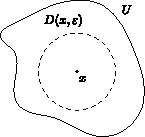
\includegraphics[scale=2]{fig/neighborhood.pdf}
	\caption{A neighborhood $U$ of $x$}
\end{figure}



\begin{prop}
	In a metric space, every $\varepsilon$-ball $D(x,\varepsilon)$ is open for $\varepsilon>0$.
\end{prop}
\begin{proof}
	Let $y \in D(x,\varepsilon)$, then $d(x,y)<\varepsilon$. Set
	 \[
		 r= \frac{\varepsilon-d(x,y)}{2}.
	\] 
	Now let $z \in D(y,r)$, then
	 \begin{align*}
		 d(x,z) &\leq d(x,y) + d(y,z) \\
			&< d(x,y) + \frac{\varepsilon-d(x,y)}{2} \\
			&= \frac{\varepsilon+d(x,y)}{2} \\
			&< \varepsilon.
	\end{align*}
	Thus there exists $D(y,r) \subset D(x,\varepsilon)$ for any $y \in D(x,\varepsilon)$, so $D(x,\varepsilon)$ is open.
\end{proof}

\begin{prop}
	In $(M,d)$ with open sets $U_i$,
	\begin{enumerate}
		\item $\bigcap_{i=1}^N U_i$ is open
		\item $\bigcup_{\alpha \in A} U_\alpha$ is open
		\item $\varnothing$ and $M$ are open
	\end{enumerate}
\end{prop}
\begin{proof}
	\begin{enumerate}
		\item Let $U_1, \dots, U_N$ be open, and let $y \in \bigcap_{i=1}^N U_i$ (if we can't find such a $y_i$, then the intersection is the empty set, which is open). Then $y_i \in U_i$ for all $i$. This implies that for each $i$, there exists $r_i$ such that $D(y,r_i) \subset U_i$. Set $r=\min\left\{ r_1,\dots,r_N \right\}$, then $D(y,r) \subset D(y,r_i) \subset U_i$ for all $i$. This implies $D(y,r) \subset \bigcap_{i=1}^N U_i$, so the intersection is open.

		\item 
			Let $x \in \bigcup_{\alpha\in A}U_\alpha$, where $U_\alpha$ is open for each $\alpha$. This implies $x \in U_\beta$ for some $\beta \in A$, so there exists $r$ such that $D(x,r) \subset U_\beta \subset \bigcup_{\alpha\in A}U_\alpha$. This implies that the union is open.

		\item This is clear.
	\end{enumerate}
\end{proof}

\begin{ex}{}{}
	Let $U_n = \left( -\frac{1}{n}, \frac{1}{n} \right)$, then $\bigcap_{n=1}^\infty U_n = \left\{ 0 \right\}$, which is not open. Thus statement (1) does not hold for arbitrary collections of open sets.
\end{ex}


%%%%%%%%%%%%%%%%%%%%
% Interior of a Set
%%%%%%%%%%%%%%%%%%%%

\section{Interior of a Set}
\begin{defn}{Interior}{interior}
	If $A \subset (M,d)$, then let $A^o \doteq \left\{ x\in A \;|\; \text{there exists } D(x,\varepsilon) \subset A \right\}$
\end{defn}

\begin{ex}{}{}
	$[0,1]^o = (0,1)$.
\end{ex}

\begin{defn}{Interior Point}{int-point}
	A point $a \in A$ is an \textbf{interior point} if there's an open set $U$ such that $a \in U \subset A$. The interior of a set is all that set's interior points.
\end{defn}

The interior of $A$ is the union of all open subsets of $A$. Since $A^o$ is open, $A^o$ is the largest open subset of $A$. Thus if $A$ has no open subsets, then $A^o=\varnothing$. Furthermore, if $A$ is open, then $A^o=A$.


%%%%%%%%%%%%%%%%%%%%
% Closed Sets
%%%%%%%%%%%%%%%%%%%%

\section{Closed Sets}
\begin{defn}{Closed}{closed}
	A set $B$ in a metric space $M$ is said to be \textbf{closed} if its complement $B^c = M\backslash B$ is open.
\end{defn}
It's possible for a set to be neither open nor closed (consider $(0,1] \in \mathbb{R}$).

\begin{prop}
        In $(M,d)$ with open sets $C_i$,
        \begin{enumerate}
                \item $\bigcup_{i=1}^N U_\alpha$ is closed
                \item $\bigcap_{\alpha\in A} C_\alpha$ is closed
                \item $\varnothing$ and $M$ are closed
        \end{enumerate}
\end{prop}
\begin{proof}
	The proofs of the first two statements follow almost immediately from DeMorgan's laws, so we can prove those first. Let $\{F_\alpha\}$ be a collection of closed sets. Write $F_\alpha=U_\alpha^c$ for open $U_\alpha$. Then $\cup_\alpha F_\alpha =\cup_\alpha U_\alpha^c$.

	Let $x \in \cup_\alpha U_\alpha^c$, then $x\in U_\beta^c$ for some $\beta$ and, subsequently, $x \not\in U_\beta$. This implies $x \not\in \cap_\alpha U_\alpha$, so $x \in \left( \cap_\alpha U_\alpha \right)^c$.

	Now let $y \in \left( \cap_\alpha U_\alpha \right)^c$, then $y \not\in \bigcap_\alpha U_\alpha$. Then $y \not\in U_\beta$ for some $\beta$, so $y \in U_\beta^c$. This means $y \in \cup_\alpha U_\alpha^c$.

	These two implications combine to give $\cup_\alpha U_\alpha^c = \left( \cap_\alpha U_\alpha \right)^c$. Similarly, we can derive $\cap_\alpha U_\alpha^c = \left( \cup_\alpha U_\alpha \right)^c$. With DeMorgan's laws proven, we can move on to the proofs of the statements we actually care about.

	\begin{enumerate}
		\item The intersection of finite open sets is open, so $\cup_{j=1}^N F_j = \left( \cap_{j=1}^N U_j \right)^c$ must be closed by definition.
		\item The union of an arbitrary collection of open sets is open, so $\cap_\alpha F_\alpha = \left( \cup_\alpha U_\alpha \right)^c$ must be closed by definition.
		\item $\varnothing$ and $M$ are each other's complements, and they are both open. Thus by definition they are both also closed.
	\end{enumerate}

\end{proof}

\begin{ex}{}{}
Any finite set in $\mathbb{R}^n$ is closed since it is the union of finitely many single points, which themselves are closed sets.
\end{ex}

\begin{ex}{}{}
	Let \[F_n = \left[\frac{1}{n}, 1-\frac{1}{n}\right] .\] The union $\bigcup_{j=1}^\infty F_j = (0,1)$, so the union of an arbitrary collection of closed sets is not necessarily closed.
\end{ex}

%%%%%%%%%%%%%%%%%%%%
% Accumulation Points
%%%%%%%%%%%%%%%%%%%%

\section{Accumulation Points}
\begin{defn}{Accumulation Point}{acc-point}
	A point $x$ in metric space $M$ is an \textbf{accumulation point} of $A \subset M$ if every open set $U$ containing $x$ contains some point of $A$ other than $x$. Equivalently, for all $\varepsilon>0$, $D(x,\varepsilon)$ contains $y\in A$ such that $y\neq x$. This can also be written $\left(D(x,\varepsilon) \backslash \left\{ x \right\}\right) \cap A \neq \varnothing$.

	The set of accumulation points of $A$ is denoted by $\text{acc}(A)$.
\end{defn}

Other points of $A$ get arbitrarily close to $x$ if $x$ is an accumulation point. This means there are infinitely many points of $A$ that are close to $x$.

An accumulation point of a set doesn't need to be in the set itself. A set also doesn't need to have any accumulation points in the first place.

\begin{figure}[H]
	\centering
	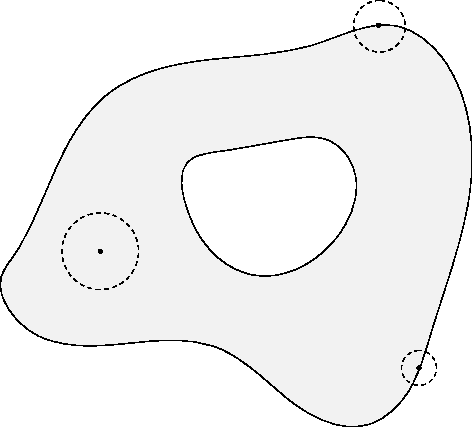
\includegraphics[scale=1]{fig/accumulation-pt.pdf}
	\caption{Accumulation points of a set}
\end{figure}


\begin{ex}{}{}
	\begin{enumerate}
		\item Let $S \subset \mathbb{R}$ be bounded, and let $x$ be a least upper bound of $S$. Let $D(x,\varepsilon)$ be the $\varepsilon$-ball around $x$, then if $D(x,\varepsilon) \cap S = \varnothing$, then $x - \varepsilon/2$ is an upper bound for $S$. This is a contradiction, so $D(x,\varepsilon) \cap S \neq \varnothing$, meaning $x$ is an accumulation point of $S$.
		\item Discrete metric spaces have no accumulation points.
	\end{enumerate}
\end{ex}

\begin{prop}
	Every point in $A^o$ is an accumulation point of $A \subset \mathbb{R}^n$.
\end{prop}
\begin{proof}
	Let $x \in A^o$, then there exists $\varepsilon>0$ such that $D(x,\varepsilon) \subset A^o \subset A$. Then $(D(x,\varepsilon) \backslash \{x\}) \cap A$ is nonempty.
\end{proof}

\begin{prop}
	\label{acc-closed}
	$A \subset (M,d)$ is closed if and only if the accumulation points of $A$ belong to $A$.
\end{prop}
\begin{proof}
	\textbf{Forward:} Let $F \subset (M,d)$ be closed, and let $x \in F^c$. Since $F^c$ is open, there exists $\varepsilon>0$ such that $D(x,\varepsilon) \subset F^c$. This implies $D(x,\varepsilon) \cap F = \varnothing$, so $x$ is \textit{not} an accumulation point of $F$. Thus $F$ contains all its accumulation points.

	\textbf{Backward:} Let $F \subset (M,d)$ be a set which contains its accumulation points. Let $p \in F^c$, then it is \textit{not} an accumulation point of $F$. Then there exists an open neighborhood $U$ of $p$ such that $U \cap F = \varnothing$. Then there exists $\varepsilon>0$ such that $D(p,\varepsilon) \subset U \subset F^c$, so $F^c$ is open, so $F$ is closed.
\end{proof}

If a set has no accumulation points, then it satisfies this condition and is thus closed.


%%%%%%%%%%%%%%%%%%%%
% Closure of a Set
%%%%%%%%%%%%%%%%%%%%

\section{Closure of a Set}
\begin{defn}{Closure}{closure}
	Let $A \subset (M,d)$, then $\overline{A}$ is the intersection of all closed sets containing $A$. It is the smallest closed set containing $A$.
\end{defn}

Since the intersection of any family of closed sets is closed, $\overline{A}$ is closed.

\begin{prop}
	For $A \subset M$, $\bar{A}=A \cup \text{acc}(A)$.
\end{prop}
\begin{proof}
	Let $B=A \cup \text{acc}(A)$. By Proposition \ref{acc-closed}, any closed set containing $A$ also contains $B$. If $B$ is closed, then it will be therefore be the smallest closed set containing $A$, i.e. $B = \overline{A}$. To show that $B$ is closed, we use Proposition \ref{acc-closed} again.

	Let $y$ be an accumulation point of $B$. If $\varepsilon>0$, then $D(y,\varepsilon)$ contains other points of $B$. Let $z \in B$ be one of them, then either $z \in A$ or $ z \in \text{acc}(A)$. In the latter case, $D(z, \varepsilon-d(z,y))$ is an open set containing $z$, and so by definition it must contain other points of $A$ that are distinct from $y$. Thus $y$ is also an accumulation point of $A$, so $y \in B$. This implies that $B$ is closed and, subsequently, equal to the closure of $A$.
\end{proof}


%%%%%%%%%%%%%%%%%%%%
% Boundary of a Set
%%%%%%%%%%%%%%%%%%%%

\section{Boundary of a Set}
\begin{defn}{Boundary}{boundary}
	The \textbf{boundary} of $A \subset (M,d)$ is defined $\partial A = \overline{A}\cap \overline{A^c}$.
\end{defn}
The union of 2 closed sets is closed, so $\partial A$ is closed. Note $\partial A = \partial A^c $.

\begin{prop}
	Let $A \subset M$, then $x \in \partial A$ if and only if for all $\varepsilon>0$, $D(x,\varepsilon)$ contains points of $A$ and $A^c$ (these points might include $x$ itself).
\end{prop}
\begin{proof}
	\textbf{Forward:} Let $x \in \partial A$. If $x \in A$, then it must be an accumulation point of $A^c$. If $x \in A^c$, then it must be an accumulation point of $A$. Either way, the conclusion follows.

	\textbf{Backward:}  The same cases apply here, and the argument is similar.
\end{proof}

$x \in \partial A$ need not be an accumulation point.

\begin{ex}{}{}
	\begin{enumerate}
		\item Let $A=(0,1)$, then $\overline{A}=[0,1]$ and $\overline{A^c} =(-\infty,0] \cup[1,\infty)$. Then $\partial A = \{0,1\}$.
		\item Let $A=\mathbb{Q}$, then $\overline{A}=\mathbb{R}$. $A^c = \mathbb{R}\backslash \mathbb{Q}$, so $\overline{A_c} = \mathbb{R}$. Thus $\partial \mathbb{Q}=\mathbb{R}$.
	\end{enumerate}
\end{ex}


%%%%%%%%%%%%%%%%%%%%
% Sequences in Metric Spaces
%%%%%%%%%%%%%%%%%%%%

\section{Sequences in Metric Spaces}
\begin{defn}{Convergence}{conv}
	A sequence $\left\{ x_n \right\}_{n=1}^\infty \subset (M,d)$ \textbf{converges} to $L \in M$ if for all $\varepsilon>0$, there exists some $N$ such that if $n>N$, then  $d(x_n,L)<\varepsilon$.

	Equivalently, $x_n\to L$ if for every open neighborhood $U$ of $L$, there exists $N$ such that if $n>N$, then $x_n \in U$.
\end{defn}

Like a good mathematician, you gotta prove that these two definitions are actually equivalent.
\begin{proof}
	\textbf{First implies second:} Let $U$ be an open neighborhood of $L$, then there exists $\varepsilon>0$ such that $D(L,\varepsilon) \subset U$. We know that there exists $N$ such that if $n>N$, then $d(x_n,L)<\varepsilon$, which implies $x_n \in D(L,\varepsilon)$, which itself implies $x\in U$.

	\textbf{Second implies first:} Fix $\varepsilon>0$, then $D(L,\varepsilon)$ is an open neighborhood of $L$. Then there exists $N$ such that for $n>N$, $x_n \in D(L,\varepsilon)$. This implies $d(x_n, L) < \varepsilon$.
\end{proof}

\begin{ex}{}{}
	For the discrete metric, a sequence $\left\{ x_n \right\}$ converges if and only if it is constant for big enough $n$.
\end{ex}

Some of the properties of limit arithmetic also carry over into the more general case, as well.
\begin{prop}
	If $(\mathcal{V},\Vert{\cdot}\Vert)$ is a normed vector space and $\left\{ v_k \right\}, \left\{ w_k \right\} \subset \mathcal{V}$ such that $v_k \to v$ and $w_k \to w$, and if $\left\{ \lambda_k \right\} \subset \mathbb{R}$ such that $\lambda_k \to \lambda$, then
	\begin{enumerate}
		\item $v_k + w_k \to v+w$
		\item $\lambda_k v_k \to \lambda v$
	\end{enumerate}
\end{prop}
The proofs of these don't really change when we go from $\mathbb{R}$ to $\mathcal{V}$, so hopefully you put the proofs for the earlier limit arithmetic properties in these notes somewhere.

A corollary of this is $w_k \to w \iff w_k - w \to 0$ for all sequences in normed vector spaces.

\begin{prop}
	$F\subset (M,d)$ is closed if an only if for all sequences in $F$ that converge to a point in $M$, that point is also in $F$.
\end{prop}
\begin{proof}
	\textbf{Forward:} Let $F$ be closed, and let $\left\{ x_n \right\}\subset F$ such that $x_n \to L \in M$. Then every neighborhood of $L$ contains elements of $F$. This implies that $L$ is an accumulation point of $F$. Since $F$ is closed, it contains its accumulation points. Thus $L \in F$.

	\textbf{Backward:} Suppose that every sequence $\left\{ x_n \right\}\subset F$ satisfies  $x_n \to L \in M \implies L \in F$. Let $p$ be an accumulation point of $F$, then for all $n$, we have $D(p,1/n) \cap F \neq \varnothing$. This means we can find a point $x_n \in D(p,1/n) \cap F$. By construction, $x_n \to p$. By assumption, this implies $p \in F$. Then $F$ contains its accumulation points, so $F$ is closed.
\end{proof}

\begin{prop}
	For a set $A \subset (M,d)$, $x \in \overline{A}$ if and only if there is a sequence $x_k \in A$ with $x_k \to x$.
\end{prop}
\begin{proof}
	This argument is similar to the previous proof.
\end{proof}

\begin{ex}{}{}
	Consider the open interval $(0,1)$ with the usual metric. The sequence $\left\{ 1/n \right\}$ does \textit{not} converge in this metric space since $0 \not\in M$.
\end{ex}

\begin{prop}
	$v_k \to v$ in $\mathbb{R}^n$ if and only if each sequence of coordinates converges to the corresponding coordinate of $v$ as a sequence in $\mathbb{R}$. That is, $\lim v_k = v$ in $\mathbb{R}^n$ if and only if $\lim v_k^i = v^i$ in $\mathbb{R}$ for each $i=1,2,\dots,n$.
\end{prop}
\begin{proof}
	\textbf{Forward:} If $\delta(v,v_k) = \max\left\{ |v^1-v_k^1|, \dots, |v^n-v_k^n| \right\}$, then $\delta(v,v_k) \leq \Vert{v-v_k}\Vert \leq \sqrt{n} \delta(v,v_k)$ (see Proposition \ref{root-thing}). Suppose $v_k \to v$ in $\mathbb{R}^n$ and $1 \leq j \leq n$. Let $\varepsilon>0$, then there is an integer $K$ such that $\Vert{v-v_k}\Vert<\varepsilon$ whenever $k \geq K$. Therefore, for such $k$, we have $|v^j - v_k^j| \leq \delta(v,v_k) \leq \Vert{v-v_k}\Vert<\varepsilon$, and so $v_k^j \to v^j$ in $\mathbb{R}$.

	\textbf{Backward:} Suppose that for each $j=1,\dots,n$, we have $\lim v_k^j = v^j$. Let $\varepsilon>0$, then for any $\varepsilon_0>0$, there are integers $K_1,K_2,\dots,K_n$ such that
	\begin{gather*}
		|v^1 - v_k^1| < \varepsilon_0 \text{ whenever } k \geq K_1 \\
		|v^2 - v_k^2| < \varepsilon_0 \text{ whenever } k \geq K_2 \\
			      \vdots \\
		|v^n - v_k^n| < \varepsilon_0 \text{ whenever } k \geq K_n
	\end{gather*}
	There are only finitely many $K_i$, so one of them is the largest. Let $K= \max(K_1,\dots,K_n)$. For $k \geq K$, we know $\Vert{v-v_k}\Vert \leq \sqrt{n} \delta(v,v_k) < \sqrt{n} \varepsilon_0$. If this is done with $\varepsilon_0=\varepsilon/\sqrt{n} $, we obtain $\Vert{v-v_k}\Vert<\varepsilon$ whenever $k \geq K$, and so $v_k \to v$ in $\mathbb{R}^n$.
\end{proof}


%%%%%%%%%%%%%%%%%%%%
% Complete Metric Spaces
%%%%%%%%%%%%%%%%%%%%

\section{Complete Metric Spaces}
\begin{defn}{Cauchy Sequence}{cauchy}
	The sequence $\left\{ x_n \right\}\subset (M,d)$ is a \textbf{Cauchy sequence} if for all $\varepsilon>0$, there exists $N$ such that if $n,m>N$, then $d(x_n,x_m) < \varepsilon$.
\end{defn}

Unlike convergence, Cauchy sequences are metric-dependent. There's no real way to define them in terms of open neighborhoods. {\color{red}This is what the prof said, but that doesn't seem right?} 

\begin{defn}{Completeness}{comp}
	A metric space $(M,d)$ is \textbf{complete} if every Cauchy sequence in $M$ converges.
\end{defn}

\begin{ex}{}{}
	\begin{enumerate}
		\item $\mathbb{R}^n$ is complete.
		\item Any discrete metric space is complete.
	\end{enumerate}
\end{ex}

\begin{defn}{Bounded}{bounded}
	A set $A \subset (M,d)$ is \textbf{bounded} if there exists some $p \in M$ and $R>0$ such that $A \subset D(p,R)$.

	A sequence is bounded if and only if its image is bounded (remember that we defined sequences to be functions, so their image is the set of all points in the sequence).
\end{defn}

\begin{figure}[H]
	\centering
	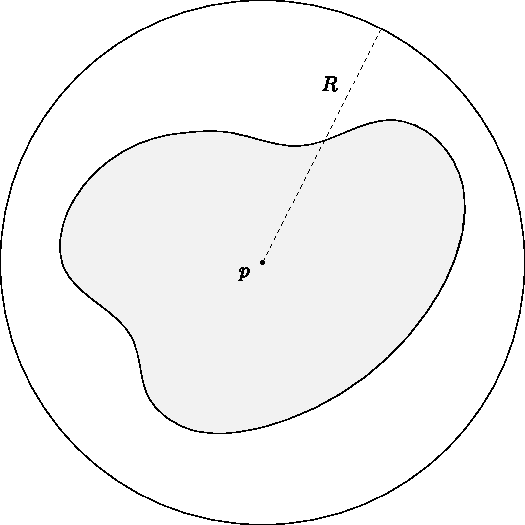
\includegraphics[scale=0.7]{fig/bounded.pdf}
	\caption{A bounded set}
\end{figure}


\begin{prop}
	A convergent sequence in a normed vector space or metric space is bounded.
\end{prop}
\begin{proof}
	If $x_n  \to x$, then there exists $N$ such that $d(x_n , x) < 1$ whenever $n > N$. Thus for all $n > N$, $x_n \in D(x,1)$. Let $M = \max\left\{ d(x_1,x), \dots, d(x_{N},x), 1 \right\}$, then $d(x_i, x) \leq M$ for all $i$.
\end{proof}

\begin{prop}
	Just as in $\mathbb{R}$, we can develop some properties of Cauchy sequences.
	\begin{enumerate}
		\item Every convergent sequence in a metric space is a Cauchy sequence.
		\item A Cauchy sequence in a metric space is bounded.
		\item If a subsequence of a Cauchy sequence converges to $x$, then the sequence converges to $x$.
	\end{enumerate}
\end{prop}
\begin{proof}
	The proofs of these are essentially the same as the proofs for $\mathbb{R}$, except absolute values are replaced with distances.
\end{proof}

\begin{ex}{}{}
	Consider $(0,\infty)$ with metric $d(x,y) = | \ln(x/y) | $. This space is complete (although it's \textit{not} complete under the usual metric). Now define $f:(0,\infty) \leftrightarrow \mathbb{R}$ by $x \mapsto \ln x$, then $|f(x)-f(y)|=|\ln x - \ln y| = |\ln (x/y)|$.

	Since $\mathbb{R}$ is complete and $f$ is an isometry (the points in $\mathbb{R}$ that get mapped to are the same distance away as the original points in our interval), then the space $(0,\infty)$ with metric $|\ln(x/y)|$ is complete.
\end{ex}

\begin{thrm}{}{}
	A sequence $\left\{ x_k \right\} \subset \mathbb{R}^n$ converges to a point in $\mathbb{R}^n$ if and only if it is a Cauchy sequence.
\end{thrm}
\begin{proof}
	\textbf{Forward:} If $x_k \to x$, then for $\varepsilon>0$, choose $N$ so that $k \geq N$ implies $\Vert{x_k-x}\Vert<\varepsilon/2$. Then for $k,l \geq N$, $\Vert{x_k-x_l}\Vert=\Vert{(x_k-x)+(x-x_l)}\Vert \leq \Vert{x_k-x}\Vert+\Vert{x-x_l}\Vert < \varepsilon/2 + \varepsilon/2 = \varepsilon$. Thus $\left\{ x_k \right\}$ is a Cauchy sequence.

	\textbf{Backward:} Suppose $\left\{ x_k \right\}$ is Cauchy. Since $|x_k^i - x_l^i| \leq \Vert{x_k-x_l}\Vert$, the components are also Cauchy sequences in $\mathbb{R}$. Since $\mathbb{R}$ is complete and every Cauchy sequence in $\mathbb{R}$ converges to a point in $\mathbb{R}$, $x_k^i \to x^i$ for each $i$. Since we have pointwise convergence, we also have convergence of the full sequence $\left\{ x_k \right\}$.
\end{proof}

\begin{defn}{Cluster Point}{clus-pt}
	A point $x$ in a metric space is called a \textbf{cluster point} of $\left\{ x_k \right\}$ if for every $\varepsilon>0$, there are infinitely many values of $k$ with $d(x_k,x)<\varepsilon$.
\end{defn}

\begin{prop}
	If $\left\{ x_k \right\}\subset (M,d)$ and $x \in M$, then
	\begin{enumerate}
		\item $x$ is a cluster point if and only if for every $\varepsilon>0$ and for each integer $N$, there is a $k >N$ with $d(x_k,x) < \varepsilon$.
		\item $x$ is a cluster point if and only if there is a subsequence convergent to $x$.
		\item $x_k \to x$ if and only if every subsequence converges to $x$.
		\item $x_k \to x$ if and only if every sebsequence of $\left\{ x_k \right\}$ has a further subsequence that converges to $x$.
	\end{enumerate}
\end{prop}
\begin{proof}
	These are also analagous to the proofs for $\mathbb{R}$. I'm sensing a pattern in this section...
\end{proof}


%%%%%%%%%%%%%%%%%%%%
% Series in Normed Vector Spaces
%%%%%%%%%%%%%%%%%%%%

\section{Series in Normed Vector Spaces}

Let $(\mathcal{V},|\cdot|)$ be a normed vector space and let $\left\{ x_i \right\}_{i=1}^\infty\subset \mathcal{V}$. Set $S_n \doteq \sum_{i=1}^{n} x_i$. If $S_n \to L$, we say $\sum_{i=1}^{\infty} x_i$ is convergent and $\sum_{i=1}^{\infty} x_i = L$. If $\left\{ S_n \right\}$ does \textit{not} converge, we say $\sum_{i=1}^{\infty} x_i$ does not converge.

If $\mathcal{V}=\mathbb{R}$, we say $S_i \to \infty$ if for all $M$, there exists $N$ such that if $n  >N$, then $S_n > M$. If $S_i \to \pm \infty$, we say $\sum_{i=1}^{\infty} x_i = \pm\infty$ (respectively).

\begin{defn}{Banach Space}{}
A \textbf{Banach space} is a complete normed vector space.
\end{defn}

\begin{defn}{Hilbert Space}{}
A \textbf{Hilbert space} is a complete inner product space.
\end{defn}


\begin{thrm}{}{norm-conv}
	Let $\mathcal{V}$ be a complete normed vector space. A series $\sum x_k $ converges if and only if for every $\varepsilon>0$, there is an $N$ such that $k  >N$ implies
	\[
	\Vert{x_k + x_{k+1}+\cdots+x_{k+p}}\Vert<\varepsilon
	\] 
	for all integers $p=0,1,2,\dots$
\end{thrm}
\begin{proof}
	Let $s_k = \sum_{i=1}^{k} x_k$. Since $\mathcal{V}$ is complete, a $\left\{ s_k \right\}$ converges if and only if it is a Cauchy sequence. This is true if and only if there is an $N$ such that $l > N$ implies $\Vert{s_l - s_{l+q}}\Vert <\varepsilon$ for all $q=1,2,\dots$. But $\Vert{s_l - s_{l+q}}\Vert=\Vert{x_{l+1}+\cdots+x_{l+q}}\Vert$, and so the result follows with $k=l+1$ and $p=q-1$.
\end{proof}

\begin{thrm}{}{}
In a complete normed vector space, if $\sum x_k$ converges absolutely, then $\sum x_k$ converges.
\end{thrm}
\begin{proof}
	This follows from Theorem \ref{thrm:norm-conv} and the triangle inequality
	 \[
	\Vert{x_k + \cdots + x_{k+p}}\Vert \leq \Vert{x_k}\Vert+\cdots+\Vert{x_{k+p}}\Vert.
	\] 
\end{proof}


{\color{red}Finish this section.}


%+-------------------+
%| +---------------+ |
%| |    Chapter    | |
%| +---------------+ |
%+-------------------+
% Compact and Connected Sets

\chapter{Compact and Connected Sets}

%%%%%%%%%%%%%%%%%%%%
% Compactness
%%%%%%%%%%%%%%%%%%%%

\section{Compactness}

By ``compact", we want to convey that a set is somehow closed and bounded. The standard definition of compactness, which is equivalent to the intuitive definition when we are in $\mathbb{R}^n$, is formulated in terms of open covers.

\begin{defn}{Cover}{cover}
	A \textbf{cover} of $A \subset (M,d)$ is a collection $\left\{ U_i \right\}$ of sets whose union contains $A$. It is an \textbf{open cover} if each $U_i$ is open (in which case the union is always also open). A \textbf{subcover} of a given cover is a subcollection of $\left\{ U_i \right\}$ whose union also contains $A$ (or ``covers" $A$). A \textbf{finite subcover} is a subcover composed of only a finite number of sets.
\end{defn}

\begin{ex}{}{}
	Let $A=[0,1]$, and let $U_x = (x-1/2, x+1/2)$. The set $\left\{ U_x \right\}_{x\in A}$ is clearly an open cover of $A$. The set $\left\{ U_0,U_{1/2},U_1 \right\}$ clearly a finite subcover of $A$.
\end{ex}

\begin{defn}{Sequentially Compact}{seq-compact}
	$A \subset (M,d)$ is \textbf{sequentially compact} if every sequence in $A$ has a subsequence that converges to a point in $A$.
\end{defn}

\begin{defn}{Compact}{compact}
	$A \subset (M,d)$ is \textbf{compact} if every open cover of $A$ has a finite subcover.
\end{defn}

\begin{figure}[H]
	\centering
	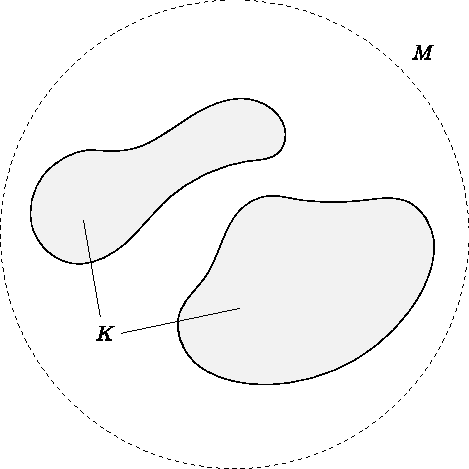
\includegraphics[scale=0.75]{fig/compact.pdf}
	\caption{An intuitive depiction of what a compact set $K \subset (M,d)$ could look like}
\end{figure}


\begin{thrm}{Bolzano-Weierstrass Theorem}{BW}
	$A \subset (M,d)$ is compact if and only if $A$ is sequentially compact.
\end{thrm}
\begin{proof}
	{\color{red}Proof on page 167 of textbook.} 
\end{proof}


\begin{defn}{Totally Bounded}{tot-bounded}
	$A \subset (M,d)$ is \textbf{totally bounded} if for every $\varepsilon>0$, there is a finite set $\left\{ x_1,\dots,x_{N(\varepsilon} \right\} \subset M$ such that \[A \subset \bigcup_{i=1}^{N(\varepsilon)} D(x_i,\varepsilon).\]
\end{defn}

\begin{prop}
	A compact set is closed.
\end{prop}
\begin{proof}
	Let $K$ be compact, let $x \in K^c$, and let $U_n = \left\{ y \;|\; d(y,x) > 1/n \right\}$. Then $\left\{ U_n \right\}_{n=1}^\infty$ covers $\left\{ x \right\}^c$, so it also covers $K$. Since $K$ is compact, there is a finite number of these open sets that cover it. Since $U_n \subset U_{n+1}$, there is a single $U_N$ of this finite subcover that covers $K$ by itself. Then $K \subset \left\{ y \;|\; d(x,y) > 1/N \right\}$, which implies $D(x,1/N) \subset K^c$. Thus $K_c$ is open and, subsequently, $K$ is closed.
\end{proof}

\begin{prop}
	A closed subset of a compact set is compact.
\end{prop}
\begin{proof}
	Let $K$ be compact and $A \subset K$ be closed, and let $\mathcal{U}$ be a collection of open sets that acts as an open cover of $A$. Since $A$ is closed, $A^c$ is open, so $\mathcal{U} \cup \{A^c\}$ is an open cover of $K$. Then there exists a finite subcover $\mathcal{U}' \cup \{A^c\}$ of $K$. Then $\mathcal{U}'$ covers $A$. Since $\mathcal{U}'$ is finite and was derived from an arbitrary open cover, $A$ is compact.
\end{proof}

\begin{prop}
	A sequentially compact set is totally bounded.
\end{prop}
\begin{proof}
	We can prove this by contradiction. Let $A$ be sequentially compact, and suppose it is not totally bounded. Then there is some $\varepsilon>0$ such that $A$ is not covered by a finite number of $\varepsilon$-balls. Now let
	\begin{align*}
		y_1 &\in A \\
		y_2 &\in A \backslash D(y_1,\varepsilon) \\
		    &\vdots \\
		y_{n+1} &\in A \backslash \bigcup_{j=1}^n D(y_j, \varepsilon)
	\end{align*}
	We can always find a $y_j$ in each of the above sets since $A$ is assumed to not be totally bounded.

	Since $A$ is sequentially compact, there exists a subsequence $y_{\sigma(j)}$ such that $y_{\sigma(j)}\to y \in A$. This means the subsequence is Cauchy, i.e. there exists $N$ such that $d(y_{\sigma(j)}, y_{\sigma(k)}) < \varepsilon/2$ for any $\varepsilon>0$ when $\sigma(j),\sigma(k) > N$. But we constructed each $y_j$ to be at least $\varepsilon$ away from all other $y_j'$. Thus by contradiction, $A$ is totally bounded.
\end{proof}

\begin{prop}
	A compact set is bounded.
\end{prop}
\begin{proof}
	Let $A \subset (M,d)$ be compact, then $A \subset \bigcup_{j=1}^\infty D(0,j)$. Since $A$ is compact, we must be able to find a finite subcover $\bigcup_{k=1}^N D(0,j_k)$ of $A$. Since $D(0,k) \subset D(0,l)$ when $k<l$, this implies that $D \subset D(0, j')$ for $j' = \min\left\{ j_1, \dots, j_N \right\}$.
\end{proof}

\begin{thrm}{}{}
	$(M,d)$ is compact if and only if $M$ is complete and bounded. Similarly, $A \subset (M,d)$ is compact if and only if $A$ is closed and bounded.
\end{thrm}
\begin{proof}
	{\color{red}Get proof from book.} 
\end{proof}


\begin{defn}{Finite Intersection Property}{FIP}
	A collection of closed sets $\left\{ K_\alpha \right\}$ in a metric space $M$ has the \textbf{finite intersection property} for $A$ if the intersection of any finite number of the $K_\alpha$ with $A$ is nonempty.
\end{defn}

\begin{prop}
	$A \subset (M,d)$ is compact if and only if every collection of closed sets with the finite intersection property for $A$ has nonempty intersection with $A$.
\end{prop}
\begin{proof}
	\textbf{Forward:} Assume $A$ is compact. Let $\left\{ F_i \right\}$ be a collection of closed setes and let $U_i = F_i^c$, so that $U_i$ is open. Suppose $A \cap ( \cap_{i=1}^\infty F_i) = \varnothing$. Taking complements, this means that $\left\{ U_i \right\}$ covers $A$. Since the cover is open, there is a finite subcover, say, $A \subset U_1 \cup \cdots \cup U_N$. Then $A \cap (F_1 \cap \cdots \cap F_N) = \varnothing$. This implies that $\left\{ F_i \right\}$ doesn't have the finite intersection property. Thus $A \cap \left\{ F_i \right\} \neq \varnothing$ for any finite collection $\left\{ F_i \right\}$ satisfying the finite intersection property.

	\textbf{Backward:} Let $\left\{ U_i \right\}$ be an open cover of $A$ and let $F_i = U_i^c$. Then $A \cap (\cap_{i=1}^\infty F_i) = \varnothing$, and so, by assumption, $\left\{ F_i \right\}$ cannot have the finite intersection property for $A$. Thus $A \cap (F_1 \cap\cdots\cap F_N) = \varnothing$ for some members $F_1,\dots,F_N$ of the collection. Then $U_1,\dots,U_N$ is the required finite subcover, so $A$ is compact.
\end{proof}


%%%%%%%%%%%%%%%%%%%%
% The Heine-Borel Theorem
%%%%%%%%%%%%%%%%%%%%

\section{The Heine-Borel Theorem}

\begin{thrm}{Heine-Borel Theorem}{}
	$A \subset \mathbb{R}^n$ is compact if and only if it is closed and bounded.
\end{thrm}
\begin{proof}
	We already know that compact sets are closed and bounded (see lemmas in the proof of the Bolzano-Weierstrass theorem, Theorem \ref{thrm:BW}, so we only need to show the backward implication.

	If we show that a closed and bounded set $A$ is sequentially compact, then by Bolzano-Weierstrass, it is also compact. We will use the fact that every bounded subset of $\mathbb{R}$ has a convergent subsequence (see the Bolzano-Weierstrass property, Theorem \ref{thrm:BW-real}. Let $\left\{ x_k \right\}=\left\{ x_k^1,x_k^2,\dots,x_k^n \right\} \subset A$ be a sequence (those are superscripts, not exponents). Since $A$ is bounded, $\left\{ x_k^1 \right\}$ has a convergent subsequence, say, $\{ x_{f_1(k)}^1 \}$. Then $\{ x_{f_1(k)}^2 \}$ has a convergent subsequence, say, $\{ x_{f_2(k)}^2 \}$. Continuing, we get $\{ x_{f_n(k)} \} = \{ x_{f_n(k)}^1, \dots, x_{f_n(k)}^n \}$, all of whose components converge. Pointwise convergence in $\mathbb{R}^n$ implies overall convergence, so $\left\{ x_{f_n(k)} \right\}$ converges to some point in $\mathbb{R}^n$. Since $A$ is closed, the limit must lie in $A$. Thus $A$ is sequentially compact, and so is compact.
\end{proof}


%%%%%%%%%%%%%%%%%%%%
% Nested Set Property
%%%%%%%%%%%%%%%%%%%%

\section{Nested Set Property}
\begin{thrm}{Nested Set Property}{}
	Let $\left\{ F_k \right\}$ be a sequence of compact nonempty sets in a metric space $M$ such that $F_{k+1}\subset F_k$, then their intersection is nonempty, i.e.
	 \[
	\bigcap_{k=1}^\infty F_k \neq \varnothing.
	\] 
\end{thrm}
\begin{proof}
	Here are two proofs of this theorem.

	\textbf{Proof 1:} In the compact set $A = F_1$, the compact nonempty sets $F_1,F_2,\dots$ have the finite intersection property, since $F_1\cap\cdots\cap F_k =F_k$ and $F_k \cap A \neq \varnothing$ for any $k$. We've already proven that $A$ is compact if and only if every collection of closed sets with the finite intersection property for $A$ has nonempty intersection with $A$. Thus for any $\left\{ F_k \right\}$, we have $A \cap \left\{ F_k \right\} \neq \varnothing$.

	\textbf{Proof 2:} Pick $x_k \in F_k$ for each $k$. The set $F_1$ is compact and the sequence $\left\{ x_k \right\}$ lies in $F_1$, so by Bolzano-Weierstrass, $\left\{ x_k \right\}$ has a convergent subsequence. Since each $F_k$ is closed, the limit point must lie in all of them.
\end{proof}

This can be inverted in a sense. Let $A_k = F_k^c$, then each $U_k$ is open and $U_{k+1} \supset U_k$. Then $\cup_{k=1}^\infty U_k \neq M$. Thus if $M$ is a metric space and the open sets $U_k$ are increasing and have compact complements, then the union of all the $U_k$'s is not all of $M$. 

\begin{figure}[H]
	\centering
	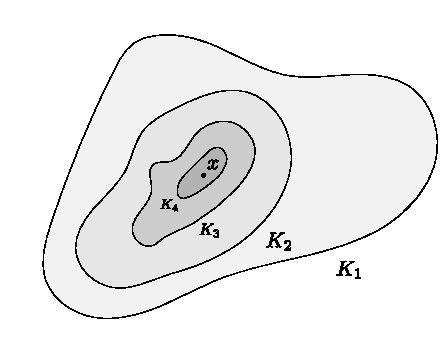
\includegraphics[scale=1]{fig/nested-set.pdf}
	\caption{As long as each $K_i$ is compact, $x$ is guaranteed to exist}
\end{figure}



%%%%%%%%%%%%%%%%%%%%
% Path-Connected Sets
%%%%%%%%%%%%%%%%%%%%

\section{Path-Connected Sets}
\begin{defn}{Continuous}{}
	For metric space  $(M,d)$, a map $\phi:[a,b]\to M$ is \textbf{continuous} if $t_k \to t$ implies $\phi(t_k) \to \phi(t)$ for every sequence $\left\{ t_k \right\} \subset [a,b]$ converging to some $t \in [a,b]$.
\end{defn}

\begin{defn}{Continuous Path}{}
	A \textbf{continuous path} joining two points $x $ and $y$ in $M$ is a mapping $\phi:[a,b] \to M$ such that $\phi(a)=x, \phi(b)=y$, and $\phi$ is continuous (here $x$ may or may not equal $y$, and $b \geq a$). A path $\phi$ \textbf{lies in a set} $A$ if $\phi(t) \in A$ for all $t \in [a,b]$.
\end{defn}

\begin{defn}{Path-Connectedness}{path-conn}
	A set is \textbf{path-connected} if every two pionts in the set can be joined by a continuous path lying in the set.
\end{defn}

A path-connected set need not be open or closed. Consider $[0,1], (0,1)$, and $[0,1)$, which are all connected.


%%%%%%%%%%%%%%%%%%%%
% Connected Sets
%%%%%%%%%%%%%%%%%%%%

\section{Connected Sets}

\begin{defn}{Connected}{}
	Let $A \subset (M,d)$, then two open sets $U,V$ \textbf{separate} $A$ if
	\begin{enumerate}
		\item $U \cap V \cap A = \varnothing$,
		\item $A \cap U \neq \varnothing$,
		\item $A \cap V \neq \varnothing$, and
		\item $A \subset U \cup V$.
	\end{enumerate}
	$A$ is \textbf{disconnected} if such sets exist, and it is \textbf{connected} if no such sets exist.
\end{defn}
{\color{red}Get rid of the $A$ in the definition maybe? Would make it seem simpler and that's what prof did.}

\begin{figure}[H]
	\centering
	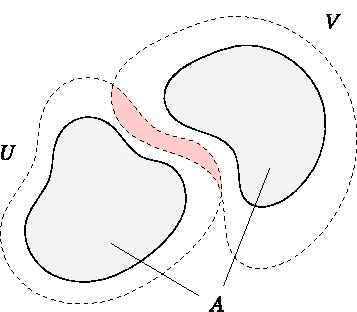
\includegraphics[scale=1]{fig/disconnected.pdf}
	\caption{A disconnected set.}
\end{figure}


\begin{prop}
	$[a,b]$ is connected.
\end{prop}
\begin{proof}
	Suppose there exists open sets $U_1,U_2$ such that $[a,b] \subset U_1 \cup U_2$, $U_1 \cap U_2 = \varnothing$, $U_1 \neq \varnothing$, and $U_2 \neq \varnothing$. Without loss of generality, assume $a \in U_1$. Since $U_1$ is open, $[a,s) \subset U_1$ for some $s > a$. We can generalize this into a set.

	Let $S \doteq \left\{ x\in [a,b] \;|\; [a,x] \subset U_1\right\}$. We know $S$ is nonempty and bounded above, so it has a supremum, which we denote by $c$. If $c=b$, then $U_2=\varnothing$, so by contradiction, $c < b$. There are now two possibilities.
	\begin{enumerate}
		\item Suppose $c \in U_1$. Since $U$ is open, there exists $\varepsilon>0$ such that $(c-\varepsilon,c+\varepsilon) \subset U_1$. This contradicts $c$ being an upper bound.
		\item Suppose $c \not\in U_1 \implies c \in U_2$. Since $U_2$ is open, there exists $\varepsilon>0$ such that $(c-\varepsilon,c+\varepsilon) \subset U_2$. Thus $c-\varepsilon$ is an upper bound of $U_1$, which contradicts $c$ being the least upper bound.
	\end{enumerate}
	Since all possibilities led to contradiction, the assumptions were false. Thus $[a,b]$ is connected.
\end{proof}

\begin{thrm}{}{}
Path-connected sets are connected.
\end{thrm}
\begin{proof}
	{\color{red}Look this up in book.}
\end{proof}

\begin{defn}{Component}{}
	A \textbf{component} of a set $A$ is a connected subset $A_0 \subset A$ such that there is no connected set in $A$ containing $A_0$ (other than $A_0$ itself). Thus a component of $A$ is a maximal connected subset of $A$.
\end{defn}

\begin{defn}{Path Component}{}
This is similar to components, except $A_0$ is the maximal path-connected subset of $A$.
\end{defn}


%+-------------------+
%| +---------------+ |
%| |    Chapter    | |
%| +---------------+ |
%+-------------------+
% Continuous Mappings

\chapter{Continuous Mappings}

%%%%%%%%%%%%%%%%%%%%
% Continuity
%%%%%%%%%%%%%%%%%%%%

\section{Continuity}

\begin{defn}{Limit of a Function}{}
Let $f: A \subset M_1 \to M_2$. Suppose that $x_0$ is an accumulation point of $A$, then $b \in M_2$ is the \textbf{limit of $f$ at $x_0$} 
\[
	\lim_{x \to x_0} f(x) = b
\] 
if given any $\varepsilon>0$, there exists $\delta>0$ such that for all $x\in A$ satisfying $x\neq x_0$ and $d_1(x,x_0)<\delta$, we have $d_2(f(x),b))<\varepsilon$.

Written in terms of open sets, this says that for all $\varepsilon>0$, there exists $\delta>0$ such that $f(D(x_0,\delta) \backslash \left\{ x_0 \right\}) \subset D(L,\varepsilon)$.
\end{defn}

The limit of a function at any given point need not exist, but when it does exist, it is unique.

\begin{prop}
	A function $f:M_1\to M_2$ is continuous if and only if for all $p \in M_1$, $\lim_{x \to p} f(x) = f(p)$.
\end{prop}
\begin{proof}
	\textbf{Forward:} Let $\varepsilon>0$, then $D(f(p), \varepsilon)$ is open in $M_2$. Since $f$ is continuous, $f^{-1}(D(f(p), \varepsilon))$ is open in $M_1$. It also contains $p$, so there exists some $\delta>0$ such that $D(p,\delta) \subset f^{-1}(D(f(p),\varepsilon))$. Thus $f(D(p,\delta)) \subset D(f(p), \varepsilon)$.

	\textbf{Backward:} Suppose $\lim_{x \to p} f(x) = f(p)$ for every $p \in M_1$. Let $U \subset M_2$, then we must show that $f^{-1}(U)$ is open. Let $p \in f^{-1}(U)$, then $f(p) \in U$. Then there exists $\varepsilon>0$ such that $D(f(p),\varepsilon) \subset U$.

	Since $f(x) \to f(p)$, apply $f^{-1}$ to both sides of the definition of the limit of a function to show that there exists $\delta>0$ such that \[D(p,\delta)\backslash\left\{ p \right\} \subset f^{-1}(D(f(p),\varepsilon)) \subset f^{-1}(U).\] Since $p \in f^{-1}(U)$, this implies that $D(p,\delta) \subset f^{-1}(U)$. Thus $f^{-1}(U)$ is open, which makes $f$ continuous.
\end{proof}

\begin{defn}{Continuity at a Point}{}
	Let $A \subset M_1$, $f:A \to M_2$, and $x_0 \in A$. We say that $f$ is \textbf{continuous at $x_0$} if either $x_0$ is not an accumulation point of $A$ or $\lim_{x \to x_0} f(x)=f(x_0)$.
\end{defn}

We can now formulate several equivalent notions of continuity over larger sets.
\begin{thrm}{Continuity}{}
	Let $f:A \subset M_1 \to M_2$, then the following are equivalent notions of continuity of $f$.
\begin{enumerate}
	\item $f$ is continuous at every point of $A$.
	\item For every convergent sequence $x_k \to x$ in $A$, we have $f(x_k) \to f(x)$.
	\item For every open set $U \subset M_2$, $f^{-1}(U)$ is open in $M_1$.
	\item For every closed set $F \subset M_2$, $f^{-1}(F)$ is closed in $M_1$.
\end{enumerate}
\end{thrm}
\begin{proof}
	This is not a proof, but we will show that if $f$ is continuous by definition 3, then definition 4 automatically holds. Let $f:M_1\to M_2$ be continuous, and let $F \subset M_2$ be closed. Then $F^c$ is open, so $f^{-1}(F)$ is open, so $f^{-1}(F)^c = f^{-1}(F^c)$ is closed. 

	{\color{red}Check the book for other stuff.}
\end{proof}

{\color{red}Redo this section with the open set defn of continuity being the main one.}

\begin{figure}[H]
	\centering
	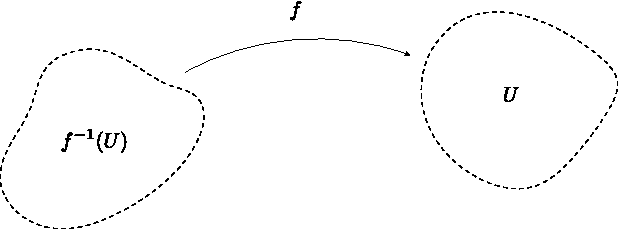
\includegraphics[scale=1]{fig/cts.pdf}
	\caption{A continuous function $f$}
\end{figure}




%%%%%%%%%%%%%%%%%%%%
% Images of Compact and Connected Sets
%%%%%%%%%%%%%%%%%%%%

\section{Images of Compact and Connected Sets}

\begin{thrm}{}{}
	Let $f:M_1 \to M_2$ be continuous, and let $K\subset M_1$ be connected. Then $f(K)$ is also connected. Similarly, if $K$ is path-connected, then $f(K)$ is also path-connected.
\end{thrm}
\begin{proof}
	We first show the result for connectedness. Assume $f(K)$ is disconnected, then there exist open $U,V$ such that
	\begin{enumerate}
		\item $f(K) \cap U \cap V = \varnothing$,
		\item $f(K) \cap U \neq \varnothing$ and $f(K) \cap V \neq \varnothing$, and
		\item $f(K) \subset U \cup V$.
	\end{enumerate}
	We will now show that $f(K)$ being disconnected results in $K$ being disconnected, a contradiction. Since $f$ is continuous, $U' \doteq f^{-1}(U)$ and $V' \doteq f^{-1}(V)$ are both open. Additionally, they cover $K$, i.e. $K \subset U' \cup V'$. It is also clear that $f^{-1}(U\cap V) = f^{-1}(U) \cap f^{-1}(V)$, so $K \cap U' \cap V' = \varnothing$. Finally, it is clear that $K \cap U'$ and $K \cap V'$ are both nonempty. Thus $K$ is disconnected, which is a contradiction, so $f(K)$ must be connected.

	We now show the path-connected result. Let $f(x) = \tilde{x}$ and $f(y) = \tilde{y}$, and let $\varphi: [a,b] \to K$ be a continuous map between $x$ and $y$, then we claim $f \circ \varphi : [a,b] \to f(K)$ is a continuous map between $\tilde{x}$ and $\tilde{y}$. It lies in $f(K)$ since $\varphi$ lies in $K$. Since $\varphi(a)=x$ and $\varphi(b)=y$, we have $f(\varphi(a))=\tilde{x}$ and $f(\varphi(b))=\tilde{y}$. Finally, $f \circ \varphi$ is continuous by Proposition \ref{comp-cts}, which we prove in the next section. Thus $f\circ\varphi$ is the desired map, and $f(K)$ is subsequently path-connected.
\end{proof}

\begin{thrm}{}{}
	Let $f:M_1\to M_2$ be continuous, and let $K\subset M_1$ be compact, then $f(K)$ is compact.
\end{thrm}
\begin{proof}
	Let $\left\{ U_\alpha \right\}_{\alpha\in A}$ be an open cover of $f(K)$, then $\left\{ f^{-1}(U_\alpha) \right\}_{\alpha\in A}$ is an open cover of $K$. Then there is a finite subcover $f^{-1}(U_{\alpha_1}) \cup \cdots \cup f^{-1}(U_{\alpha_N})$ of $K$, and since $f$ is continuous, this subcover is open. Thus $f(K)$ is covered by the finite subcover $U_{\alpha_1} \cup \cdots \cup U_{\alpha_N}$.
\end{proof}

\begin{ex}{}{}
	Consider $f:(0,\infty) \to \mathbb{R}$ defined by $f(x) = 1/x$. The preimage of the compact set $[-1,1]$ is $f^{-1}([-1,1]) = [1,\infty)$, which is not compact. So the preimages of compact sets aren't necessarily compact under continuous maps, only the images.
\end{ex}


%%%%%%%%%%%%%%%%%%%%
% Operations on Continuous Mappings
%%%%%%%%%%%%%%%%%%%%

\section{Operations on Continuous Mappings}

If $f:m_1\to M_2$ is continuous and $M_2$ is a normed vector space, then the usual limit arithmetic theorems apply.

\begin{prop}
	\label{comp-cts}
	Let $f_1:M_1 \to M_2$ and $f_2:M_2 \to M_3$ be continuous, then their composition $f_2 \circ f_1: M_1 \to M_3$ is also continuous.
\end{prop}
\begin{proof}
	Let $U \subset M_3$ be open, then $(f_2 \circ f_1)^{-1}(U) = f_1^{-1}(f_2^{-1}(U))$. Since $f_2$ is continuous, $f_2^{-1}(U)$ is open. Since $f_1$ is continuous, $f_1^{-1}(f_2^{-1}(U))$ is open.
\end{proof}

{\color{red}Stuff on page 185 of textbook.}

{\color{red}Product metric.}

\begin{prop}
	Let $\mathcal{V}$ be a normed vector space and equip $\mathcal{V} \times \mathcal{V}$ with the product metric, then
	\begin{enumerate}
		\item $+:\mathcal{V}\times \mathcal{V} \to \mathcal{V}$ is continuous
		\item $\cdot:\mathbb{R} \times \mathcal{V} \to \mathcal{V}$ is continuous
	\end{enumerate}
\end{prop}
\begin{proof}
	\begin{enumerate}
		\item Let $U \subset \mathcal{V}$ be open. Let $(v,w) \in +^{-1}(U)$, i.e. $v+w \in U$, then there exists $\varepsilon>0$ such that $D(v+w,\varepsilon) \subset U$. We want to find $\delta>0$ such that $+(D( (v,w), \delta)) \subset D(v+w,\varepsilon)$. If we can find such a $\delta$, then we will have a $\delta$-ball (an open set) within the preimage of $U$. Since this open ball is being constructed for an arbitrary member of the preimage, the preimage must then be open.

			Let $(x,y) \in D( (v,w), \delta)$, then $d( (x,y), (v,w) ) < \delta$. This is equivalent to $\Vert{x-v}\Vert+\Vert{y-w}\Vert<\delta$ since $\mathcal{V}\times \mathcal{V}$ is equipped with the product metric. By the triangle inequality,
			\[
				d(x+y,v+w) = \Vert{x+y - (v+w)}\Vert \leq \Vert{x-v}\Vert+\Vert{y-w}\Vert < \delta.
			\] 
			Let $\delta=\varepsilon$, then $+(D( (v,w), \delta)) \subset D(v+w,\varepsilon) \subset U$. Thus $D( (v,w), \delta) \subset +^{-1}(U)$ and, subsequently, $+^{-1}(U)$ is open.

		\item Similar.
	\end{enumerate}
\end{proof}

\begin{cor}
	If $(M,d)$ is a metric space, $\mathcal{V}$ is a normed vector space, and $f:M\to \mathcal{V}$, $g:M\to \mathcal{V}$, and $h:M \to \mathbb{R}$ are continuous, then
	\begin{enumerate}
		\item $f+g$ is continuous, and
		\item $hf$ is continuous.
	\end{enumerate}
\end{cor}
\begin{proof}
	Both proofs use the strategy of decomposing the operations into compositions of functions that we know to be continuous.
	\begin{enumerate}
		\item Since $f$ and $g$ are continuous, then $(f,g):M\times M \to \mathcal{V} \times \mathcal{V}$ defined by $(f,g)(x,y) = (f(x), g(y))$ is continuous. Addition is continuous, so $+ \circ (f,g): M\times M \to \mathcal{V}$ is continuous. Define $\Delta:M \to M\times M$ by $\Delta(x) = (x,x)$. This is clearly continuous, so $+ \circ (f,g) \circ \Delta = f+g$  is continuous.
		\item The composition $\cdot \circ (h,f) \circ \Delta$ is continuous.
	\end{enumerate}
\end{proof}

%%%%%%%%%%%%%%%%%%%%
% The Boundedness of Continuous Functions on Compact Sets
%%%%%%%%%%%%%%%%%%%%

\section{The Boundedness of Continuous Functions on Compact Sets}

\begin{thrm}{Maximum-Minimum Theorem}{max-min}
	Let $(M,d)$ be a metric space, let $A \subset M$, let $f:A \to \mathbb{R}$ be continuous, and let $K \subset A$ be compact. Then $f$ is bounded on $K$, i.e. $B = \left\{ f(x) \;|\; x\in K \right\}$ is a bounded set. Furthermore, there exists $x, y \in K$ such that $f(x) = \inf(B)$ and $f(y) = \sup(B)$.
\end{thrm}
\begin{proof}
	Since $K$ is compact and $f$ is continuous, $f(K)$ is compact, so it is also closed and bounded. Since it's closed, it contains its accumulation points. Its infimum and supremem are either in the set or accumulation points, so they must lie in $f(K)$.
\end{proof}


%%%%%%%%%%%%%%%%%%%%
% The Intermediate Value Theorem
%%%%%%%%%%%%%%%%%%%%

\section{The Intermediate Value Theorem}

\begin{thrm}{Intermediate Value Theorem}{}
	Let $A \subset (M,d)$, and let $f:A \to \mathbb{R}$ be continuous. Suppose that $K \subset A$ is connected and $x,y \in K$. Then for every real number $c \in \mathbb{R}$ such that $f(x) < c < f(y)$, there exists a point $z \in K$ such that $f(z) = c$.
\end{thrm}
\begin{proof}
	Suppose no such $z$ exists, then $f(A) \subset (-\infty,c) \cup (c, \infty)$. Since $y_1 < c$ and $y > c$, we know both sets in this union are nonempty. Since $f(A)$ is then clearly covered by two disjoint nonempty sets, it is disconnected. Since $A$ was taken to be path-connected (and thus also connected), this is a contradiction, so such a $z$ actually does exist.
\end{proof}

\begin{figure}[H]
	\centering
	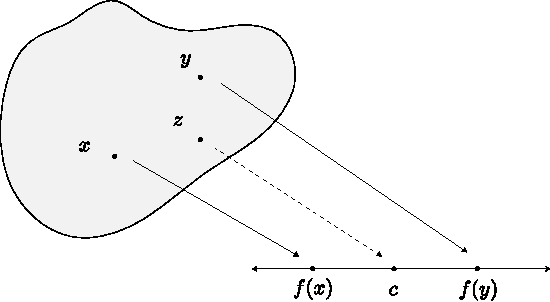
\includegraphics[scale=0.8]{fig/intermediate-value.pdf}
	\caption{The Intermediate Value Theorem}
\end{figure}


%%%%%%%%%%%%%%%%%%%%
% Uniform Continuity
%%%%%%%%%%%%%%%%%%%%

\section{Uniform Continuity}
\begin{defn}{Uniform Continuity}{}
	Let $(M_1,d_1)$ and $(M_2,d_2)$ be metric spaces, and let $f:M_1 \to M_2$ be any function. We say that $f$ is \textbf{uniformly continuous} if for all $\varepsilon>0$ and for all $x,y \in M_1$, there exists $\delta>0$ such that if $d_1(x,y) < \delta$, then $d_2(f(x), f(y)) < \varepsilon$.
\end{defn}

It should be clear how to restrict the uniform continuity of $f$ to certain sets. If $x,y \in A \subset M_1$ and the above condition holds, then $f$ is uniformly continuous on $A$.

Note that unlike usual continuity, we have to find a $\delta$ that works for \textit{all} $x$ and $y$, so it must be independent of the inputs to the function.

\begin{ex}{}{}
	Let $f:\mathbb{R}\to\mathbb{R}$ be defined by $f(x) = x^2$. Consider \[|f(x)-f(y)| = |x^2-y^2| = |(x+y)(x-y)| < \varepsilon,\]
	then $|x-y| < \varepsilon/|x+y|$. Since the difference between points needed to satisfy the $\varepsilon$ constraint depends on the inputs themselves, $f$ is \textit{not} uniformly continuous.
\end{ex}

Observe that if we had been working in a compact set instead of all of $\mathbb{R}$, $|x+y|$ would have been bounded and then $f$ \textit{would} have been uniformly continuous. This observation is formalized in the next theorem.

\begin{thrm}{Uniform Continuity Theorem}{}
Let $f:M_1\to M_2$ be continuous and let $K \subset M_1$ be compact, then $f$ is uniformly continuous on $K$.
\end{thrm}
\begin{proof}
	Given $\varepsilon>0$ and $x \in K$, choose $\delta_x$ such that if $d_1(x,y) < \delta_x$, then $d_2(f(x), f(y)) < \varepsilon/2$ (we can find such $\delta_x$ because $f$ is continuous). Then $\left\{ D(x,\delta_x/2) \right\}$ is an open cover of $K$. Since $K$ is compact, there is a finite subcover $\left\{ D(x_1,\delta_{x_1}/2), \dots, D(x_N,\delta_{x_N}/2) \right\}$. Let $\delta = \min\left\{ \delta_{x_1}/2, \dots, \delta_{x_N}/2 \right\}$.

	If $d_1(x,y) < \delta$, then there is an $x_i$ such that $d_1(x,x_i) < \delta_{x_i}/2$ (since the disks cover $K$). Then by the triangle inequality,
	\[
		d_1(x_i,y) \leq d_1(x,x_i) + d_1(x,y) < \delta_{x_i}.
	\] 
	Thus for any $x,y \in K$ such that $d_1(x,y) < \delta$,
	\[
		d_2(f(x),f(y)) \leq d_2(f(x), f(x_i)) + d_2(f(x_i),f(y)) < \varepsilon/2 + \varepsilon/2 = \varepsilon.
	\] 
\end{proof}


%%%%%%%%%%%%%%%%%%%%
% Differentiation of Functions of One Variable
%%%%%%%%%%%%%%%%%%%%

\section{Differentiation of Functions of One Variable}
\begin{defn}{Derivative}{}
The \textbf{derivative} of a function $f$ at point $x$ is defined
\[
	f'(x) \doteq \lim_{h \to 0} \frac{f(x+h)-f(x)}{h}.
\] 
\end{defn}

\begin{defn}{Differentiable}{}
	Let $f$ be defined on some open interval containing $x \in \mathbb{R}$. The function $f$ is \textbf{differentiable} at $x$ if $f'(x)$ exists.

	Equivalently,
	\[
		\lim_{h \to 0} \frac{f(x+h) - f(x) -f'(x) h}{h} = 0.
	\] 
	A function is differentiable on a set $A$ if it is differentiable at every point $A$.
\end{defn}

We can rewrite the definition for differentiability that avoids the issue of division by a term that approaches 0: for any $\varepsilon>0$, there is a $\delta>0$ such that if $|\Delta x|< \delta$, then
\[
	|f(x + \Delta x) - f(x) - f'(x) \Delta x| \leq \varepsilon |\Delta x|.
\] 

\begin{defn}{Big-O Notation}{}
	Let $\phi,g:(0,a) \to \mathbb{R}$. We say $\phi$ is $\mathcal{O}(g)$ if
	 \[
		 \left|\frac{\phi(x)}{g(x)} \right|
	 \] is bounded in some ``deleted'' neighborhood of 0, i.e. it lies in $D(0,r)\backslash\left\{ 0 \right\}$ for some $r>0$.

	 Additionally, we say $\phi$ is $o(g)$ if \[\lim_{x \to 0} \frac{\phi(x)}{g(x)} = 0.\]
\end{defn}

Based on these definitions, we can see that $f$ is differentiable at $x$ if there exists some $L \in \mathbb{R}$ such that $f(y)-f(x)-L(y-x)$ is $o(|y-x|)$.

\begin{defn}{Lipschitz}{}
	A function $f:M_1\to M_2$ is \textbf{Lipschitz} if there exists some $L \geq 0$ such that $d_2(f(x), f(y)) \leq L d_1(x,y)$ for all $x,y \in M_1$. The function $f$ is \textbf{locally Lipschitz} if for every compact set $K \subset M_1$, $f$ restricted to $K$ is Lipschitz.
\end{defn}

Note that any Lipschitz function is also \textit{uniformly} continuous. If we want $d_2(f(x),f(y))$ be to less than some $\varepsilon>0$, then take $x$ and $y$ such that $d_1(x,y) < \varepsilon/L$.

\begin{prop}
	If $f$ is differentiable at $x$, then $f$ is continuous at $x$.
\end{prop}
\begin{proof}
	\textbf{Version 1:} 
	Recall that a function $f$ is continuous at $x$ if and only if $\lim_{x_k \to x} f(x_k) = f(x)$. This is the case because
	\begin{align*}
		\lim_{x_k \to x} f(x_k) &= \lim_{x_k \to x} \left[ f(x_k) - f(x) + f(x) \right] \\
					&= \lim_{x_k \to x} \left[ \frac{f(x_k) - f(x)}{x_k - x} (x_k - x) + f(x) \right] \\
					&= f'(x) \cdot 0 + f(x) \\
					&= f(x).
	\end{align*}
	So since $f$ is differentiable at $x$, it is also continuous at $x$.

	\textbf{Version 2:}
	This version uses the second definition of differentiability. Given $\varepsilon>0$, there is a $\delta>0$ such that
	\[
		|f(x+\Delta x) - f(x) - f'(x) \Delta x| \leq \varepsilon|\Delta x|
	\] 
	if $|\Delta x| < \delta$. Then by the triangle inequality,
	\[
		|f(x+\Delta x) - f(x)| \leq |f'(x) \Delta x| + \varepsilon|\Delta x|.
	\] 
	Choosing $\varepsilon=1$,
	\[
		|f(x+\Delta x)-f(x)| \leq (f'(x)+1)|\Delta x|
	\] 
	if $|\Delta x| < \delta$. This shows that $f$ has the Lipschitz property at $x$, from which continuity follows.
\end{proof}

\begin{figure}[H]
	\centering
	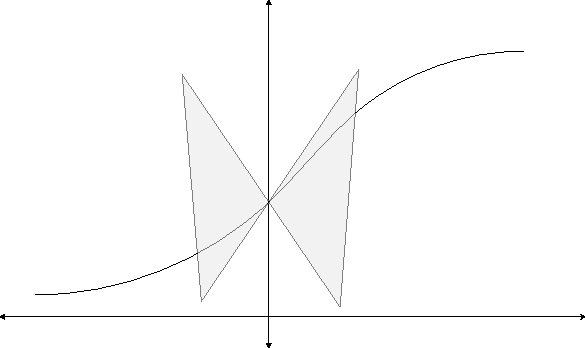
\includegraphics[scale=1]{fig/lipschitz.pdf}
	\caption{The Lipschitz property for a real-valued one variable function}
\end{figure}

\begin{thrm}{}{}
Suppose that $f$ and $g$ are differentiable at $x$ and that $k \in \mathbb{R}$, then $kf$, $f+g$, and $fg$ are differentiable at $x$ with the expected derivatives.
\begin{enumerate}
	\item $(kf)'(x) = kf'(x)$
	\item $(f+g)'(x) = f'(x) + g'(x)$
	\item $(fg)'(x) = f'(x) g(x) + f(x) g'(x)$
\end{enumerate}
\end{thrm}
\begin{proof}
	\begin{enumerate}
		\item {\color{red}Do this.}
		\item {\color{red}Do this.}
		\item {\color{red}Do this.}
	\end{enumerate}
\end{proof}

\begin{thrm}{Chain Rule}{}
	If $f$ is differentiable at $x$ and $g$ is differentiable at $f(x)$, then $g \circ f$ is differentiable at $x$ and
	\[
		(g \circ f)'(x) = g'(f(x)) f'(x)
	\] 
\end{thrm}
\begin{proof}
	{\color{red}find in textbook.}
\end{proof}

\begin{defn}{Differentiability Class}{}
	If $f$ is differentiable on $(a,b)$ and $f'$ is continuous, we say that $f$ is of \textbf{class} $C^1$. If $f'$ is differentiable and $f''$ is continuous, we say that $f$ is of class $C^2$.

More generally, if $f^{(n-1)}$ is differentiable and $f^{(n)}$ continuous, $f$ is of class $C^{n}$. The function $f$ is of class $C^{\infty}$ if it is infinitely differentiable. 
\end{defn}


\begin{defn}{Increasing and Decreasing Functions}{}
	A function $f$ defined in a neighborhood of $x$ is \textbf{increasing} at $x$ if there is an interval $(a,b)$ containing $x$ such that
	\begin{enumerate}
		\item If $a < y < x$, then $f(y) \leq f(x)$, and
		\item If $x < y < b$, then $f(y) \geq f(x)$.
	\end{enumerate}
	Similarly, $f$ is \textbf{decreasing} at $x$ if there is an interval $(a,b)$ containing $x$ such that
	\begin{enumerate}
		\item If $a < y < x$, then $f(y) \geq f(x)$, and
		\item If $x < y < b$, then $f(y) \leq f(x)$.
	\end{enumerate}
	Strictly increasing and decreasing functions are defined by making the above inequalities strict.
\end{defn}


\begin{thrm}{}{}
Let $f$ be differentiable at $x$, then
\begin{enumerate}
	\item If $f$ is increasing at $x$, then $f'(x) \geq 0$,
	\item If $f$ is decreasing at $x$, then $f'(x) \leq 0$,
	\item If $f'(x) > 0$, then $f$ is strictly increasing at $x$, and
	\item If $f'(x) < 0$, then $f$ is strictly decreasing at $x$.
\end{enumerate}
\end{thrm}
\begin{proof}
	{\color{red}Prove this.}
\end{proof}

\begin{prop}
	\label{der-slope-0}
	If $f:(a,b) \to \mathbb{R}$ is differentiable at $c \in (a,b)$ and if $f$ has a maximum (or minimum) at $c$, then $f'(c) = 0$.
\end{prop}
\begin{proof}
	If $f'(c) > 0$, then $f$ is strictly increasing at $c$, which is a contradiction. If $f'(c) < 0$, then $f$ is strictly decreasing at $c$, which is also a contradiction. Thus $f'(c)=0$.
\end{proof}

We can combine this with the maximum-minimum theorem (Theorem \ref{thrm:max-min}) to yield the familiar Rolle's Theorem.

\begin{thrm}{Rolle's Theorem}{rolle}
	If $f:[a,b] \to \mathbb{R}$ is continuous, $f$ is differentiable on $(a,b)$, and $f(a) = f(b) = 0$, then there is a number $c \in (a,b)$ such that $f'(c) = 0$.
\end{thrm}
\begin{proof}
	If $f(x) = 0$ for all $x \in [a,b]$, we can choose any $c$. Therefore assume that $f$ is not identically zero. From the maximum-minimum theorem (Theorem \ref{thrm:max-min}), we know that there is a point $c_1$ where $f$ assumes its maximum and there is a point $c_2$ where $f$ assumes its minimum. Since $f$ is not identically zero and $f(a)=f(b)=0$, at least one of $c_1,c_2$ lies in $(a,b)$. If $c_1 \in (a,b)$, then $f'(c_1)=0$ by Proposition \ref{der-slope-0}. The same is true if $c_2 \in (a,b)$.
\end{proof}

\begin{thrm}{Mean Value Theorem}{mean-val}
	If $f:[a,b] \to \mathbb{R}$ is continuous and differentiable on $(a,b)$, there is a point $c \in (a,b)$ such that $f(b) - f(a) = f'(c) (b-a)$.
\end{thrm}
\begin{proof}
	Let \[\varphi(x) = f(x)-f(a)-(x-a)\frac{f(b)-f(a)}{b-a}, \]
	then apply Rolle's Theorem.
\end{proof}

\begin{figure}[H]
	\centering
	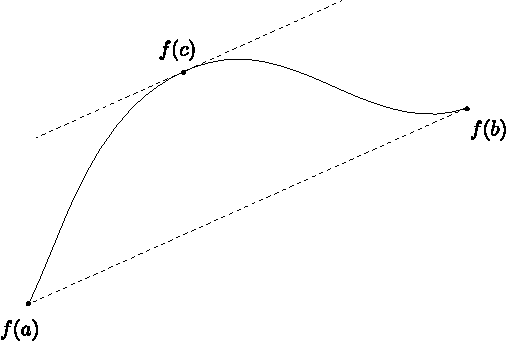
\includegraphics[scale=1]{fig/mean-value.pdf}
	\caption{The Mean Value Theorem}
\end{figure}


\begin{cor}
	\label{cor:der-constant}
	If $f:[a,b] \to \mathbb{R}$ is continuous and if $f'=0$ on $(a,b)$, then $f$ is constant.
\end{cor}
\begin{proof}
	Applying the mean value theorem to $f$ gives a point $c$ such that $f(b)-f(a) = f'(c)(b-a) = 0$, so $f(a) = f(b)$ for all $x \in [a,b]$. Thus $f$ is constant.
\end{proof}

\begin{cor}
	If $f:(a,b)\to\mathbb{R}$ is differentiable with $|f'(x)|\leq M$ for every $x \in (a,b)$, then $|f(x)-f(y)| \leq M |x-y|$ for all $x,y \in (a,b)$, i.e. $f$ is $M$-Lipschitz.
\end{cor}
\begin{proof}
	For any $x,y$, the mean value theorem gives us a point $c \in (x,y)$ such that $|f(b)-f(a)| = |f'(c) (b-a)| \leq M |b-a|$.
\end{proof}

{\color{red}I don't know if I want to include proposition 4.7.14 on page 202 of the textbook b/c it's very similar to theorem 19. I could probably combine them to save room.}

\begin{prop}
	Let $f \in C([a,b])$ be differentiable on $(a,b)$ such that $f'(x) \geq 0$ for every $x \in (a,b)$, then $f$ is increasing on $[a,b]$. If $f'(x) \leq 0$ for every $x \in(a,b)$ instead, then $f$ is decreasing on $[a,b]$.
\end{prop}
\begin{proof}
	Suppose $y>x$ and $f'\geq 0$, then for some $c \in (x,y)$, $f(y)-f(x) = f'(c) (y-x) \geq 0$ since $y-x$ is positive. Thus $f(y) \geq f(x)$, so $f$ is increasing. Similarly, $f(y) \leq f(x)$ if $f' < 0$, so $f$ is decreasing in that situation.
\end{proof}

\begin{thrm}{Inverse Function Theorem}{}
	Suppose that $f:(a,b) \to \mathbb{R}$ is either strictly increasing or strictly decreasing over $(a,b)$. Then $f$ is a bijection onto its range, $f^{-1}$ is differentiable on its domain, and $(f^{-1})'(y) = 1/f'(x)$ where $f(x) = y$.
\end{thrm}
\begin{proof}
	{\color{red}Do this.}
\end{proof}

\begin{prop}
	Suppose that $f$ is continuous on $[a,b]$ and twice differentiable on $(a,b)$ and that $x \in (a,b)$, then
	\begin{enumerate}
		\item If $f'(x) = 0$ and $f''(x) > 0$, then $x$ is a strict local minimum of $f$, and
		\item If $f'(x) = 0$ and $f''(x) < 0$, then $x$ is a strict local maximum of $f$.
	\end{enumerate}
\end{prop}
\begin{proof}
	We only prove the first statement, as the second is similar. If $f''(x) > 0$, then $f'$ is increasing at $x$, and so there is a $\delta>0$ such that $f'(y) < 0$ if $x-\delta<y<x$ and $f'(y) > 0$ if $x<y<x+\delta$. Thus  $f(y) > f(x)$ if $x-\delta<y<x$ and $f(y)>f(x)$ if $x<y<x+\delta$.
\end{proof}

{\color{red}Somewhere in here I need to say that differentiable implies uniformly continuous.}

%%%%%%%%%%%%%%%%%%%%
% Integration of Functions of One Variable
%%%%%%%%%%%%%%%%%%%%

\section{Integration of Functions of One Variable}

The integral of a function of one variable is the signed area under the curve. To define these, we'll need a notion of partitions and upper and lower sums.

\begin{defn}{Mesh}{}
The \textbf{mesh} of a partition $P =\left\{ x_1,x_2,\dots,x_N \right\}$ is defined
\[
	|P| \doteq \sup_i |x_{i+1}-x_i|.
\] 
\end{defn}

\begin{defn}{Refinement}{}
	Let $P$ and $Q$ be partitions of $[a,b]$. We say $P$ is a \textbf{refinement} of $Q$ if $Q \subset P$. We denote this by $Q \prec P$ or $P \succ Q$.
\end{defn}

Consider a bounded function $f:A \subset \mathbb{R}\to\mathbb{R}$. If $A$ is bounded, then there is some $[a,b]\supset A$. Define $f(x)=0$ if $x \in [a,b]\backslash A$. Now partition $[a,b]$ with $P=\left\{ x_0=a,x_1,\dots,x_n=b \right\}$ such that $x_0<x_1<\cdots<x_n$.

\begin{defn}{Upper/Lower Sums}{}
	The \textbf{upper sum} of $f$ over $P$ is
	\[
		U(f,P) = \sum_{i=0}^{n-1} \sup_{x\in[x_i,x_{i+1}]} f(x) (x_{i+1}-x_i).
	\] 
	Similarly, the \textbf{lower sum} is defined
	\[
		L(f,P) = \sum_{i=0}^{n-1} \inf_{x\in[x_i,x_{i+1}]} f(x) \cdot (x_{i+1}-x_i).
	\] 
\end{defn}

Note that the supremum and infimum for each subinterval exist since $f$ is bounded. Let $-M \leq f \leq M$, then
\[
	-M(b-a) \leq L(f,P) \leq U(f,P) \leq M(b-a)
\] for any partition $P$ of $[a,b]$.

\begin{prop}
	If $P \succ Q$, then $L(f,Q) \leq L(f,P) \leq U(f,P) \leq U(f,Q)$.
\end{prop}
\begin{proof}
	By induction, it suffices to consider the case that $P=Q \cup \left\{ y \right\}$, say $x_j < y < x_{j+1}$. For the lower sums we have
	\begin{align*}
		L(f,P) - L(f,Q) &= \inf_{x\in[x_j,x_{j+1}]} f(x)(y-x_j) + \inf_{x\in[y,x_{j+1}]} f(x) (x_{j+1}-y). \\
				&\quad - \inf_{x\in[x_j,x_{j+1}]} f(x) (x_{j+1}-x_{j})
		\intertext{Since the infimum over a subset is greater than or equal to the infimum over the whole set, we have}
				&\geq \inf_{x\in[x_j,x_{j+1}]} f(x) \left[ (y-x_j) + (x_{j+1}-y) + (x_{j+1}-x_j) \right].
	\end{align*}
	All the terms in brackets cancel out, leaving us with $L(f,P) - L(f,Q) \geq 0$. Thus $L(f,Q) \leq L(f,P).$ Using the fact that the supremum over a subset is less than or equal to the supremum over the whole set, we can similarly show $U(f,P) \leq U(f,Q)$.
\end{proof}

Let $P$ and $Q$ be two partitions, then neither is necessarily a subset of the other. To get around this, we note that for all $P$ and $Q$, there exists a partition $R$ which refines both, i.e. $R \succ P$ and $R \succ Q$. The set $P \cup Q$ arranged into an ordered set is one such partition.

\begin{defn}{Upper/Lower Integral}{}
Given bounded function $f:A \to \mathbb{R}$ over a bounded set $A$, define the \textbf{upper integral} by
\[
	\overline{\int_{A} } f = \inf\left\{ U(f,P) \right\}_P
\] 
and the \textbf{lower integral} by
\[
	\underline{\int_{A} } f = \sup \left\{ L(f,P) \right\}_P.
\] 
\end{defn}

\begin{defn}{Riemann Integral}{}
	A function $f$ is \textbf{Riemann integrable} if $\overline{\int_{A} } f = \underline{\int_{A} } f$. The common value $\overline{\int_{A} } f = \underline{\int_{A} } f$ is denoted by $\int_{A} f$. If $A=[a,b]$, we write
	\[ 
	\int_{A} f = \int_{a}^{b} f.
	\] 
\end{defn}

Note that this definition does \textit{not} involve any notions of smoothness or continuity.

\begin{thrm}{}{}
	Any non-increasing or non-decreasing function on $[a,b]$ is Riemann integrable on $[a,b]$.
\end{thrm}
\begin{proof}
	Without loss of generality, assume $f$ is non-decreasing. Then for any $P$, we have
	\begin{align*}
	U(f,P) - L(f,P) &= \sum_{i=0}^{N-1} \left[ \sup_{x \in [x_i, x_{i+1}]} f(x) - \inf_{x \in [x_i, x_{i+1}]} f(x) \right] (x_{i+1} - x_i).
	\intertext{Since $f$ is non-decreasing, this becomes}
			&= \sum_{i=0}^{N-1} \left( f(x_{i+1}) - f(x_i) \right) (x_{i+1}-x_i) \\
			&\leq |P| \sum_{i=0}^{N-1} \left( f(x_{i+1}) - f(x_i) \right).
			\intertext{This is a telescoping sum, so it simplifies to}
			&= |P| \left( f(b) - f(a) \right).
	\end{align*}
	So given $\varepsilon > 0$, choose $P$ such that
	\[
		|P| < \frac{\varepsilon}{f(b)-f(a)},
	\] then $U(f,P) - L(f,P) < \varepsilon$. Thus $f$ is Riemann integrable on $[a,b]$.
\end{proof}


\begin{thrm}{}{}
	If $f:[a,b]\to\mathbb{R}$ is bounded and continuous at all but finitely many points of $[a,b]$, then it is Riemann integrable on $[a,b]$.
\end{thrm}
\begin{proof}
	{\color{red}Do this.}
\end{proof}

An immediate consequence of this is that if $f$ is continuous everywhere on $[a,b]$, then it is Riemann integrable on $[a,b]$.

\begin{prop}
	\label{prop:integral-props}
	Let $f$ and $g$ be Riemann integrable on $[a,b]$, then
	\begin{enumerate}
		\item If $k\in\mathbb{R}$, then $kf$ is integrable on $[a,b]$ and $\int_{a}^{b} kf = k \int_{a}^{b} f$,
		\item $f+g$ is integrable on $[a,b]$ and $\int_{a}^{b} (f+g)=\int_{a}^{b} f+\int_{a}^{b} g$,
		\item If $f(x) \leq g(x)$ for all $x \in [a,b]$, then $\int_{a}^{b} f \leq \int_{a}^{b} g$, and
		\item If $f$ is also integrable on $[b,c]$, then it is integrable on $[a,c]$ and $\int_{a}^{c} f = \int_{a}^{b} f + \int_{b}^{c} f$.
	\end{enumerate}
\end{prop}
\begin{proof}
	{\color{red}Do this.}
\end{proof}

\begin{cor}
	The absolute value of a definite integral of $f$ is a lower bound of the definite integral of the absolute value of $f$, i.e.
	\[
		\left| \int_{a}^{b} f(x) \;dx \right| \leq \int_{a}^{b} |f(x)| \;dx.
	\] 
\end{cor}
\begin{proof}
	$-|f| \leq f \leq |f|$, so $-\int_{a}^{b} |f| \leq \int_{a}^{b} f \leq \int_{a}^{b} |f|$, which is the desired relation.
\end{proof}

\begin{prop}
	The lower definite integral of $f$ is a lower bound of the upper definite integral, i.e.
	\[
		\underline{\int_{a}^{b}} f(x) \;dx \leq \overline{\int_{a}^{b} } f(x) \;dx.
	\] 
\end{prop}
\begin{proof}
	{\color{red}Do this.}
\end{proof}

An obvious corollary of this is that if $f$ is integrable, then this inequality is \textit{not} strict.

\begin{defn}{Antiderivative}{}
	An \textbf{antiderivative} of $f:[a,b] \to \mathbb{R}$ is a continuous function $F:[a,b]\to\mathbb{R}$ such that $F$ is differentiable on $(a,b)$ and $F'(x)=f(x)$ for $x\in(a,b)$.
\end{defn}

\begin{thrm}{The Fundamental Theorem of Calculus}{}
	Let $f:[a,b]\to\mathbb{R}$ be continuous, then $f$ has an antiderivative $F$ and
	\[
		\int_{a}^{b} f(x) \;dx = F(b)-F(a).
	\] 
	If $G$ is any other antiderivative of $f$, then we also have $\int_{a}^{b} f = G(b)-G(a)$.
\end{thrm}
\begin{proof}
	Define $F:[a,b] \to \mathbb{R}$ by $F(x) = \int_{a}^{x} f(t) \;dt$ (since $f$ is continuous, we know it is Riemann integrable). We claim that $F$ is an antiderivative of $f$. Choose $x \in (a,b)$ and $h>0$ such that $(x,x+h) \subset (a,b)$, then we have
	\begin{align*}
		\frac{F(x+h)-F(x)}{h} &= \frac{1}{h} \left( \int_{a}^{x+h} f(t)\;dt - \int_{a}^{x} f(t)\;dt \right) \\
				      &= \frac{1}{h} \left( \int_{a}^{x} f(t)\;dt + \int_{x}^{x+h} f(t)\;dt - \int_{a}^{x} f(t)\;dt \right) \\
				      &= \int_{x}^{x+h} \frac{f(t)}{h} \;dt.
	\end{align*}
	We must show that the limit of this quantity as $h\to 0$ is $f(x)$, then we'll have shown that $F$ is an antiderivative of $f$.

	Fix $\varepsilon>0$, then since $f$ is continuous, we can find $h>0$ such that
	\[
		|f(t)-f(x)|<\varepsilon
	\] when $t \in (x, x+h)$. For this $h$, we can use the identity
	 \[
		 \int_{x}^{x+h} \frac{f(x)}{h} \;dt = \frac{f(x)}{h} \int_{x}^{x+h} \;dt =  f(x)
	\] to get
	\begin{align*}
		\left| \int_{x}^{x+h} \frac{f(t)}{h} \;dt -f(x)\right| &= \left| \int_{x}^{x+h} \frac{f(t)-f(x)}{h} \;dt \right| \\
								       &\leq \int_{x}^{x+h} \frac{|f(t)-f(x)|}{h} \;dt \\
								       &< \int_{x}^{x+h} \frac{\varepsilon}{h} \;dt \\
								       &= \varepsilon.
	\end{align*}
	Thus $\lim_{h \to 0^+} (F(x+h) - F(x))/h = f(x)$. Similarly, the limit also holds from the left, so $F'(x) = f(x)$. Then from the definition of $F$ we have
	\[
		F(b) - F(a) = \int_{a}^{b} f(t) \;dt - \int_{a}^{a} f(t)\;dt = \int_{a}^{b} f(t)\;dt.
	\] 
	We must now show the uniqueness of the value of the integral. Let $G$ be any antiderivative of $f$. Since  $G'(x) = F'(x) = f(x)$ for all $x \in (a,b)$, we know
	\[
		(G-F)'(x) = f(x) - f(x) = 0
	\] for all $x \in (a,b)$. Since $F$ and $G$ are differentiable on $(a,b)$, they are continuous on $(a,b)$. {\color{red}$F$ is also apparently ``clearly" continuous at $a$ and $b$, and I'd assume the same for $G$?} Thus by Corollary \ref{cor:der-constant} of the mean value theorem, $G-F$ is constant on $[a,b]$. This means $G$ is just $F$ plus a constant (say, $C$), so
	\[
		G(b)-G(a) = F(b)+C - F(a)-C = F(b)-F(a).
	\] 
\end{proof}


%+-------------------+
%| +---------------+ |
%| |    Chapter    | |
%| +---------------+ |
%+-------------------+
% Uniform Convergence

\chapter{Uniform Convergence}

%%%%%%%%%%%%%%%%%%%%
% Pointwise and Uniform Convergence
%%%%%%%%%%%%%%%%%%%%

\section{Pointwise and Uniform Convergence}

Convergence of points is straightforward, but convergence of functions is less so. We'll define two different notions of convergence of functions, and we'll explore the implications of both. We'll see that uniform convergence is a stronger notion of convergence, and it yields the most useful properties, although sometimes pointwise convergence is all that's needed.

\begin{defn}{Pointwise Convergence}{}
	Let $X$ be a set and $M$ be a metric space. A sequence of functions $f_k : X \to M$ \textbf{converges pointwise} to $f:X \to M$ if for all $x \in X$, $f_k(x) \to f(x)$.
\end{defn}

Pointwise convergence is straightforward, but it might not preserve the properties of the $f_k$. As we can see in the next example, continuity of each $f_k$ need not translate to continuity of $f$ if we only have pointwise convergence.

\begin{ex}{}{}
Consider the sequence of sigmoid-like functions
\[
	f_k(x) = \frac{1}{1+e^{-kx}} .
\] As $k$ increases, the ``slope" of the curve near 0 gets steeper, getting closer to a vertical line. Each $f_k$ is continuous, but the sequence converges pointwise to
\[
	f(x) =
	\begin{cases}
		0 & x < 0 \\
		1/2 & x=0 \\
		1 & x>0,
	\end{cases}
\] which is clearly not continuous.
\end{ex}

\begin{defn}{Uniform Convergence}{}
	Suppose $f_k : X \to M$ is a sequence of functions such that for all $\varepsilon>0$, there is a $K$ such that $d(f_k(x), f(x)) < \varepsilon$ for all $x \in X$ when $k > K$. Then we say that $f_k$ \textbf{converges uniformly} to $f$.
\end{defn}

With uniform convergence, we have a bound on how slowly each $f_k(x)$ converges to its particular $f(x)$. As you might expect, this results in the preservation of more properties of the $f_k$. As we'll see later, if each $f_k$ is continuous or differentiable, then $f$ is continuous or differentiable, respectively.

\begin{figure}[H]
	\centering
	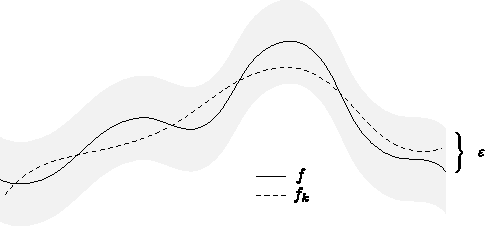
\includegraphics[scale=1.3]{fig/uniform-convergence.pdf}
	\caption{A function $f_k$ that is part of a sequence of functions converging uniformly to $f$. Note that $f_k(x)$ lies within $\varepsilon$ of $f(x)$ for all displayed values, so $k > K$ for this particular $\varepsilon$.}
\end{figure}

\begin{note}{}{}
	When $X$ is finite, both pointwise and uniform convergence are equivalent. Fix $\varepsilon>0$, then each $x_i$, there is a $K_i$ such that $|f(x_i) - f_k(x_i) | < \varepsilon$ when $k > K_i$. Since $X$ is finite, we can let $K = \max_i K_i$, then we clearly have uniform convergence.
\end{note}

\begin{defn}{Series Convergence}{}
	Let $g_k : X \to \mathcal{V}$ be a sequence of functions, where $\mathcal{V}$ is a normed vector space. We say $\sum_{k=1}^{\infty} g_k$ \textbf{converges pointwise} to $g:X \to \mathcal{V}$ if the sequence $s_n \doteq \sum_{k=1}^{n} g_k$ converges pointwise to $g$.

	Similarly, we say $\sum_{k=1}^{\infty} g_k$ \textbf{converges uniformly} to $g$ if $s_k$ converges uniformly to $g$.
\end{defn}

Note that in the above definition, we needed addition of our space's elements to make sense in order to talk about series, thus we used $\mathcal{V}$ instead of $M$.

\begin{prop}
	\label{prop:unif-cts}
	Let $f_k: M_1 \to M_2$ be a sequence of continuous functions, and let $f_k$ converge uniformly to $f$. Then $f$ is continuous on $M_1$.
\end{prop}
\begin{proof}
	Fix $\varepsilon>0$. Since $f_k$ converges uniformly to $f$, we can find a $K$ such that $d(f(x), f_k(x)) < \varepsilon/3$ when $k > K$. Since each $f_k$ is continuous, for each $k$ there is some $\delta_k > 0$ such that $d(f_k(x), f_k(y)) < \varepsilon/3$ when $d(x,y) < \delta_k$.

	Choose any $k > K$, then we have
	\begin{align*}
		d(f(x), f(y)) &\leq d(f(x), f_k(x)) + d(f_k(x), f_k(y)) + d(f_k(y), f(y)) \\
			      &< \frac{\varepsilon}{3} + \frac{\varepsilon}{3} + \frac{\varepsilon}{3} \\
			      &= \varepsilon
	\end{align*}
	when $d(x,y) < \delta_k$. Thus $f$ is continuous on $M_1$.
\end{proof}

\begin{cor}
	Let $g_k: X \to \mathcal{V}$ be continuous for all $k$. If $\sum_{k=1}^{\infty} g_k$ converges uniformly to $g$, then $g$ is continuous.
\end{cor}
\begin{proof}
	This follows from Proposition \ref{prop:unif-cts} and the fact that the sum of continuous functions is continuous (so each partial sum is continuous).
\end{proof}

\begin{note}{}{}
In other words, we can exchange limits with summations when the convergence is uniform, i.e.
\[
	\lim_{x \to x_0} \sum_{k=1}^{\infty} g_k(x) = \sum_{k=1}^{\infty} \lim_{x \to x_0} g_k(x).
\] 
\end{note}


%%%%%%%%%%%%%%%%%%%%
% The Weierstrass-M Test
%%%%%%%%%%%%%%%%%%%%

\section{The Weierstrass-M Test}

\begin{thrm}{Cauchy Criterion}{}
	Let $M$ be a complete metric space, $X$ a set, and $f_k: X \to M$ a sequence of functions. Then $f_k$ converges uniformly on $X$ if and only if for all $\varepsilon > 0$, there is a $K$ such that $d(f_k(x), f_l(x)) < \varepsilon$ for all $x \in X$ when $k,l > K$.
\end{thrm}
\begin{proof}
	{\color{red}Do this.}
\end{proof}

The Cauchy criterion can easily be rewritten to apply to series of functions instead: Let $\mathcal{V}$ be a Banach space, then $\sum_{k=1}^{\infty} g_k$ converges uniformly on $X$ if and only if for all $\varepsilon>0$, there is a $K$ such that
\[
	\Vert{g_k(x) + \cdots + g_{k+p}(x)}\Vert< \varepsilon
\] for all $x \in X$ and for all integers $p \geq 0$.

\begin{thrm}{The Weierstrass-$M$ Test}{wm-test}
	Let $\mathcal{V}$ be a Banach space, and let $g_k : X \to \mathcal{V}$ with constants $M_k$ such that
	\[
		\Vert{g_k(x)}\Vert\leq M_k
	\] for all $x \in X$ and such that $\sum_{k=1}^{\infty} M_k$ converges. Then $\sum_{k=1}^{\infty} g_k$ converges uniformly (and absolutely).
\end{thrm}
\begin{proof}
	Fix $\varepsilon>0$. Since $\sum_{k=1}^{\infty} M_k$ converges, by the Cauchy criterion there exists $N$ such that
	\[
	\Vert{M_k + \cdots + M_{k+p}}\Vert< \varepsilon
	\] for all $p \geq 0$ when $k > N$. Each $M_k \geq 0$, so this implies
	\[
	M_k + \cdots + M_{k+p} < \varepsilon.
	\] Then for $k>N$, we have
	\begin{align*}
		\Vert{g_k(x) + \cdots + g_{k+p}(x)}\Vert &\leq \Vert{g_k(x)}\Vert + \cdots + \Vert{g_{k+p}(x)}\Vert \\
		&\leq M_k + \cdots + M_{k+p}\\
		&< \varepsilon
	\end{align*}
	for all $x \in X$ and for all $p \geq 0$. Thus $\sum_{k=1}^{\infty} g_k$ converges uniformly. Since
	\[
		\big\Vert{\Vert{g_k(x)}\Vert + \cdots + \Vert{g_{k+p}(x)}\Vert}\big\Vert \leq \Vert{g_k(x)}\Vert + \cdots + \Vert{g_{k+p}(x)}\Vert < \varepsilon,
	\] it converges absolutely as well.
\end{proof}

%%%%%%%%%%%%%%%%%%%%
% Integration and Differentiation of Series
%%%%%%%%%%%%%%%%%%%%

\section{Integration and Differentiation of Series}

\begin{thrm}{}{limit-integral-exchange}
	Let $f_k$ be Riemann integrable on $[a,b] $, and suppose that they converge uniformly to some function $f$ on $[a,b]$. Then $f$ is Riemann integrable on $[a,b]$ and
	\[
		\lim_{k \to \infty} \int_{a}^{b} f_k(x) \;dx = \int_{a}^{b} f(x)\;dx.
	\] 
\end{thrm}
\begin{proof}
	First we show that $f$ is Riemann integrable. Since $f_k$ converges uniformly to $f$, for all $\varepsilon>0$ we can find a $K$ such that
	\[
		|f_k - f| < \frac{\varepsilon}{420 (b-a)} 
	\] when $k > K$. This gives us the following two inequalities:
	\begin{itemize}
		\item $\sup_x f(x) \leq \sup_x f_k(x) + \frac{\varepsilon}{420 (b-a)}$, and
		\item $\inf_x f(x) \geq \inf_x f_k(x) - \frac{\varepsilon}{420 (b-a)} $.
	\end{itemize}
	Since each $f_k$ is Riemann integrable, for all $\varepsilon>0$ we can find a $P_k$ such that
	\[
		U(f_k, P_k) - L(f_k, P_k) < \frac{\varepsilon}{420} .
	\] These two bounds give us
	\begin{align*}
		U(f, P_k) - L(P_k) &= \sum_{i=0}^{N-1} \left[ \sup_{x \in [x_i, x_{i+1}]} f(x) - \inf_{x \in [x_i, x_{i+1}]} f(x) \right] (x_{i+1}-x_i) \\
				   &\leq U(f_k, P_k) - L(f_k, P_k) + \sum_{i=0}^{N-1} \frac{\varepsilon}{210 (b-a)} (x_{i+1}-x_i) \\
				   &= U(f_k, P_k) - L(f_k, P_k) + \frac{\varepsilon}{210} \\
				   &< \frac{\varepsilon}{420} + \frac{\varepsilon}{210} \\
				   &< \varepsilon.
	\end{align*}
	Thus $f$ is Riemann integrable.

	Now we must show that $\int_{a}^{b} f = \lim_{k \to \infty} \int_{a}^{b} f_k$. Fix $\varepsilon>0$, then choose $k$ such that
	\[
		|f_k(x)-f(x)| < \frac{\varepsilon}{b-a}.
	\] for all $x$. Then
	\begin{align*}
		\left| \int_{a}^{b} f_k - \int_{a}^{b} f \right| &= \left| \int_{a}^{b} (f_k-f) \right| \\
								 &\leq \int_{a}^{b} |f_k-f| \\
								 &< \int_{a}^{b} \frac{\varepsilon}{b-a} \\
								 &= \varepsilon.
	\end{align*}
	Thus $\int_{a}^{b} f = \lim_{k \to \infty} \int_{a}^{b} f_k$.
\end{proof}

\begin{cor}
	Let $g_k : [a,b] \to \mathbb{R}$ be Riemann integrable, and suppose $\sum_{k=1}^{\infty} g_k$ converges uniformly on $[a,b]$. Then
	\[
		\int_{a}^{b} \sum_{k=1}^{\infty} g_k = \sum_{k=1}^{\infty} \int_{a}^{b} g_k.
	\] 
\end{cor}
\begin{proof}
	Apply the previous theorem to the sequence of partial sums. We can do this because the sum of a finite number of Riemann integrable functions is itself Riemann integrable (see Proposition \ref{prop:integral-props}).
\end{proof}

\begin{thrm}{}{}
	Let $f_k:(a,b) \to \mathbb{R}$ be differentiable on $(a,b)$, and suppose that $f_k$ converges pointwise to $f:(a,b) \to \mathbb{R}$. Also suppose that $f_k'$ is continuous and converges uniformly to some $g$. Then $f$ is differentiable and $f'=g$.
\end{thrm}
\begin{proof}
	Let $a<x_0<b$, then by the fundamental theorem of calculus,
	\[
		f_k(x) - f_k(x_0) = \int_{x_0}^{x} f_k'(t) \;dt.
	\] 
	Let $k \to \infty$, then since $f_k$ converges pointwise, we have
	\[
		f(x) - f(x_0) = \lim_{k \to \infty} \int_{x_0}^{x} f_k'(t)\;dt.
	\] 
	Since $f_k'$ converges uniformly, we can use Theorem \ref{thrm:limit-integral-exchange}on the integral term to get
	\[
		f(x) - f(x_0) = \int_{x_0}^{x} g(t)\;dt.
	\] 
	Since $f_k'$ converges uniformly and each  $f_k'$ is continuous, we know $g$ is also continuous. Thus by the fundamental theorem of calculus, the RHS has derivative $g(x)$. The derivative of the LHS is $f'(x)$, so we have $f'(x) = g(x)$.
\end{proof}

\begin{cor}
	\label{cor:series-differentiation}
	Let $g_k$ be differentiable with $g_k'$ continuous, and suppose that $\sum_{k=1}^{\infty} g_k$ converges pointwise and $\sum_{k=1}^{\infty} g_k'$ converges uniformly, then
	\[
		\left( \sum_{k=1}^{\infty} g_k \right)' = \sum_{k=1}^{\infty} g_k'.
	\] 
\end{cor}

\begin{ex}{}{}
	Consider \[ \frac{1}{1-x} = \sum_{k=0}^{\infty} x_k\] for $x \in (-1, 1)$. By the Weierstrass-$M$ test, $\sum_{k=0}^{\infty} x^k$ and $\sum_{k=1}^{\infty} k x^{k-1}$ converge uniformly on $[-a,a]$ for any $a <1$. Thus by Corollary \ref{cor:series-differentiation},
	\[
		\frac{d }{d x} \frac{1}{1-x} = \frac{1}{(1-x)^2} = \sum_{k=1}^{\infty} k x^{k-1}.
	\] 
\end{ex}




%%%%%%%%%%%%%%%%%%%%
% The Elementary Functions
%%%%%%%%%%%%%%%%%%%%

\section{The Elementary Functions}

{\color{red}Bruh you gotta do this.}



%%%%%%%%%%%%%%%%%%%%
% The Space of Continuous Functions
%%%%%%%%%%%%%%%%%%%%

\section{The Space of Continuous Functions}

Let $M$ be a metric space and $\mathcal{V}$ be a normed vector space, and let $\mathcal{F}$ be the set of all functions from $M$ to $\mathcal{V}$. If we define addition and scalar multiplication in the obvious ways for functions, then since the zero function is in $\mathcal{F}$, $\mathcal{F}$ is a vector space.

\begin{defn}{The Space of Continuous Functions}{}
We define the space of continuous functions between a metric space and normed vector space by
\[
	\mathcal{C}(M,\mathcal{V}) = \left\{ f \in \mathcal{F} \;|\; f \text{ continuous} \right\}.
\] 
\end{defn}

$\mathcal{C}$ is also a vector space, since it is closed under addition and scalar multiplication.

\begin{defn}{The Space of Bounded Continuous Functions}{}
We define the space of \textbf{bounded} continuous functions between a metric space and normed vector space by
\[
	\mathcal{C}_b(M, \mathcal{V}) = \left\{ f \in \mathcal{C}(M, \mathcal{V}) \;|\; f \text{ bounded} \right\}.
\] 
\end{defn}

If $M$ is compact, then by the minimum-maximum theorem, $\mathcal{C}_b = \mathcal{C}$ (each continuous function achieves its minimum and maximum, so each is bounded).

When working with $\mathcal{C}_b$, the usual norm is the supremum norm. I won't use any notation from this, since it should be obvious when something inside a norm is a function.

\begin{thrm}{}{}
\begin{enumerate}
	\item Let $M_1$ and $M_2$ be metric spaces, then so is $\mathcal{C}_b(M_1,M_2)$, i.e. the distance function $d(f,g) \doteq \sup_{x\in M_1} d_2(f(x), g(x))$ satisfies
		\begin{enumerate}
			\item $d(f,g) \geq 0$,
			\item $d(f,g) = 0 \iff f=g$,
			\item $d(f,g) = d(g,f)$, and
			\item $d(f,g) \leq d(f,h) + d(h,g)$.
		\end{enumerate}

	\item If $M$ is a metric space and $\mathcal{V}$ is a normed vector space, then $\mathcal{C}_b(M,\mathcal{V})$ is a normed vector space, i.e. the supremum norm satisfies
		\begin{enumerate}
			\item $\Vert{f}\Vert\geq 0$,
			\item $\Vert{f}\Vert=0 \iff f=0$,
			\item $\Vert{\lambda f}\Vert = |\lambda| \Vert{f}\Vert$, and
			\item $\Vert{f+g}\Vert\leq \Vert{f}\Vert+\Vert{g}\Vert$.
		\end{enumerate}
\end{enumerate}
\end{thrm}
\begin{proof}
	\begin{enumerate}
		\item The first three properties are straightforward. As usual, the only one we have to put effort into showing is the triangle inequality. For all $x \in M_1$, we have
			\[
				d_2(f(x), g(x)) \leq d_2(f(x), h(x)) + d_2(h(x), g(x))
			\] since $M_2$ is a metric space. Thus
			\begin{align*}
				d(f,g) &\leq \sup_{x \in M_1}d_2(f(x), h(x)) + d_2(h(x), g(x)) \\
				&\leq \sup_{x \in M_1}\left\{d_2(f(x), h(x))\right\} + \sup_{x \in M_1}\left\{d_2(h(x), g(x))\right\} \\
				&= d(f,h) + d(h,g).
			\end{align*}

		\item Once again, the first three properties are straightforward, but we have to show the triangle inequality. We have
			\begin{align*}
				\Vert{f+g}\Vert &= \sup_{x \in M}\Vert{f(x)+g(x)}\Vert \\
						&\leq \sup_{x \in M}\Vert{f(x)}\Vert+ \Vert{g(x)}\Vert \\
						&\leq \sup_{x}\left\{\Vert{f(x)}\Vert\right\}+ \sup_x \left\{\Vert{g(x)}\Vert\right\} \\
						&= \Vert{f}\Vert+ \Vert{g}\Vert.
			\end{align*}
	\end{enumerate}
\end{proof}


\begin{thrm}{}{}
{\color{red}$f_k$ converges uniformly to $f$ on $M$ if and only if $f_k \to f$ in $\mathcal{C}_b$}
\end{thrm}
\begin{proof}
	{\color{red}Idek what this is trying to say.}
\end{proof}

\begin{thrm}{}{}
	If $M_2$ is a complete metric space, then so is $\mathcal{C}_b(M_1,M_2)$. If $\mathcal{V}$ is a Banach space, then so is $\mathcal{C}_b(M, \mathcal{V})$.
\end{thrm}
\begin{proof}
	Let $\{f_k\} \subset \mathcal{C}_b(M_1, M_2)$ be uniformly Cauchy. Then for fixed $x$, the sequence $\{f_k(x)\}$ is Cauchy. Since $M_2$ is complete, $f_k(x) $ converges to some point in $M_2$. Call this point $f(x)$. Doing this for every $x$ defines a function $f:M_1 \to M_2$.

	We claim that $f_k$ converges uniformly to $f$. We'll use the following two facts:
	\begin{enumerate}
		\item Since $\{f_k\}$ is uniformly Cauchy, for all $\varepsilon>0$, there is a $K$ such that $d(f_m(x), f_n(x)) < \varepsilon/2$ for all $x$ when $m,n > K$.
		\item By construction, $f_k$ converges pointwise to $f$. Fix $x$, then for all $\varepsilon>0$, there is a $K_x$ such that $d(f_k(x), f(x)) < \varepsilon/2$ when $k > K_x$.
	\end{enumerate}

	Let $k > K$, then for all $m \in \mathbb{N}$ and for all $x$, we have
	\[
		d(f_k(x), f(x)) \leq d(f_k(x), f_m(x)) + d(f_m(x), f(x)).
	\] For fixed $x$, if we take $m > \max\left\{ K, K_x \right\}$, then we have
	\[
	d(f_k(x), f(x)) < \frac{\varepsilon}{2} + \frac{\varepsilon}{2} = \varepsilon.
\] At first glance, it might seem like this doesn't help because our bound uses $K_x$, which depends on $x$; however, all we needed to do was find a $K$ such that $d(f_k, f)<\varepsilon$ at all $x$ when $k > K$, and we did just that. The proof that the inequality holds is different for each $x$, but it holds for all of them nonetheless. It's a bit wack, but it works.

	Now we have to show that $f$ is in $\mathcal{C}_b(M_1, M_2)$. Since each $f_k$ is continuous and the convergence is uniform, $f$ is continuous. Now let $\varepsilon=1$, then there is some $k$ such that $d(f,g) = \sup_x d_2(f_k(x), f(x)) < 1$. Since $f_k$ is bounded, we know $d_2(f_k(x), y) \leq L$ for some $L \geq 0$ and for some $y \in M_2$. Then for this same $y$ and for all $x \in M_1$, we have
	\[
		d_2(f(x), y) \leq d_2(f(x), f_k(x)) + d_2(f_k(x), y) \leq 1 + L,
	\] so $f$ is bounded. Since $f$ is continuous and bounded, it is in $\mathcal{C}_b(M_1, M_2)$, so $\mathcal{C}_b(M_1,M_2)$ is complete.

	The second assertion can be proven in the same way, except with norms instead of distance functions.
\end{proof}

\begin{note}{}{}
The previous theorem has an inuitive analogue for $\mathcal{C}$ instead of $\mathcal{C}_b$. The proof is essentially the same, except we don't have to show that $f$ is bounded.
\end{note}


%%%%%%%%%%%%%%%%%%%%
% The Arzela-Ascoli Theorem
%%%%%%%%%%%%%%%%%%%%

\section{The Arzela-Ascoli Theorem}

\begin{defn}{Equicontinuous}{}
	Let $\mathcal{B} \subset \mathcal{C}(M_1, M_2)$. We say that $\mathcal{B}$ is \textbf{equicontinuous} if for all $\varepsilon>0$, there is a $\delta>0$ such that $d(f(x), f(y)) < \varepsilon$ for all $f \in \mathcal{B}$ when $d(x,y) < \delta$.
\end{defn}

\begin{prop}
	Let $\mathcal{B} \subset C^1(\mathbb{R},\mathbb{R})$. Suppose there is an $M \geq 0$ such that $\Vert{f'}\Vert_{\sup} \leq M$ for all $f \in \mathcal{B}$, then $\mathcal{B}$ is equicontinuous.
\end{prop}
\begin{proof}
	By the mean value theorem, $f(x) - f(y) = f'(c) (x-y) \leq M (x-y)$ for all $f \in B$. Set $\delta = \varepsilon/M$, then equicontinuity follows.
\end{proof}

\begin{defn}{Precompact}{}
A set is \textbf{precompact} if its closure is compact.
\end{defn}

\begin{thrm}{Arzela-Ascoli}{}
	Let $M_1$ be compact, and let $\mathcal{B} \subset \mathcal{C}(M_1, M_2)$. Then $\mathcal{B}$ is compact if and only if $\mathcal{B}$ is equicontinuous and pointwise precompact.
\end{thrm}
\begin{proof}
	{\color{red}Do this.}
\end{proof}

\begin{cor}
	Let $M$ be compact, and let $\mathcal{B}\subset \mathcal{C}(M, \mathbb{R}^n)$ be equicontinuous and pointwise bounded. Then every sequence in $\mathcal{B}$ has a uniformly convergent subsequence.
\end{cor}
\begin{proof}
	Fix $x$, then $\mathcal{B}_x \doteq \left\{ f(x) \;|\; f \in \mathcal{B} \right\}$ is bounded (this is the definition of pointwise bounded). Then th closure of $\mathcal{B}_x $ is closed and bounded in $\mathbb{R}^n$, so it is compact. Thus $\mathcal{B}$ is pointwise precompact.

	Since we were already given that $\mathcal{B}$ is equicontinuous and $M$ is compact, by Arzela-Ascoli we know that $\mathcal{B}$ is compact. Then every sequence in $\mathcal{B}$ has a convergent subsequence. Convergence here is with respect to the supremum norm, so the convergence is uniform.
\end{proof}


%%%%%%%%%%%%%%%%%%%%
% The Banach Fixed Point Theorem
%%%%%%%%%%%%%%%%%%%%

\section{The Banach Fixed Point Theorem}

\textit{This is also called the Contraction Mapping Principle.}

\begin{thrm}{Banach Fixed Point Theorem}{}
	Let $M$ be a complete metric space, and let $\phi:M \to M$ be $k$-Lipschitz with $k < 1$. Then there is a unique fixed point of $\phi$.
\end{thrm}
\begin{proof}
	Let $x_0 \in M$, then inductively define $x_{n+1} = \phi(x_n)$. We claim that $\left\{ x_n \right\}$ is Cauchy. Assume $n>m$, then we have
	\begin{align*}
		d(x_n, x_m) &= d(\phi(x_{n-1}), \phi(x_{m-1})) \\
			    &\leq k d(x_{n-1}, x_{m-1}) \\
			    &\vdots \\
			    &\leq k^m d(x_{n-m}, x_0).
	\end{align*}
	Additionally,
	\begin{align*}
		d(x_{n-m}, x_0) &\leq d(x_{n-m},x_{n-m-1}) + \cdots + d(x_1, x_0) \\
				&\leq \left( k^{n-m-1} + \cdots + k^0 \right) d(x_1, x_0) \\
				&\leq d(x_1, x_0) \sum_{j=0}^{\infty} k^j \\
				&= d(x_1,x_0) \frac{1}{1-k},
	\end{align*}
	where the last equality follows from $|k| < 1$ making the series geometric. Thus the distance between points $x_n$ and $x_m$ has the bound
	\[
		d(x_n, x_m) \leq d(x_1,x_0) \frac{k^m}{1-k} .
	\] This is clearly Cauchy, so since $M$ is complete, $x_n \to x^*$ for some $x^* \in M$. We must show that this limit point is a fixed point of $\phi$. By the inductive definition of our sequence, we have
	\begin{align*}
		\phi(x_n) &= x_{n+1}.
		\intertext{Taking limits of both sides gives}
		\lim_{n \to \infty} \phi(x_n) &= x^*.
		\intertext{Since $\phi$ is Lipschitz, it is continuous, so we can move the limit inside the function to get}
		\phi(x^*) &= x^*,
	\end{align*}
	so $x^*$ is a fixed point of $\phi$. We now show that $x^*$ is unique. Suppose $y^*$ is another distinct fixed point of $\phi$, then
	\begin{align*}
		d(x^*, y^*) = d(\phi(x^*), \phi(y^*)) \leq k d(x^*, y^*).
	\end{align*}
	Since $x^* \neq y^*$, this implies that $1 \leq k$, which is a contradiction. Thus $x^*$ is unique.
\end{proof}

\begin{note}{}{}
	The use of $ k$ in the Banach fixed point theorem is very important. If
	\[
		d(\phi(x), \phi(y)) < d(x,y),
	\] it might be possible to contruct a sequence of $x$'s and $y$'s such that
	\[
		d(\phi(x), \phi(y)) \to d(x,y).
	\] In this case, we won't necessarily have a fixed point. If we instead have a fixed $k$ such that
	\[
	d(\phi(x), \phi(y)) < k d(x,y),
	\] this aberrant behavior goes away.
\end{note}


%%%%%%%%%%%%%%%%%%%%
% The Stone-Weierstrass Theorem
%%%%%%%%%%%%%%%%%%%%

\section{The Stone-Weierstrass Theorem}

\begin{defn}{Algebra}{}
An \textbf{algebra} is a vector space $\mathcal{V}$ equipped with a bilinear function \[\cdot : \mathcal{V} \times \mathcal{V} \to \mathcal{V}.\]
\end{defn}

Suppose $\mathcal{B}$ is an algebra. If $f,g \in \mathcal{B}$ and $\alpha$ is a scalar, then $fg$, $f+g$, and $\alpha f$ are all in $\mathcal{B}$.

\begin{defn}{Separates Points}{}
	A set of functions $\mathcal{B}$ \textbf{separates points} if, for $x \neq y$, there is some function $f \in \mathcal{B}$ such that $f(x) \neq f(y)$.
\end{defn}

\begin{thrm}{Stone-Weierstrass}{}
	Let $M$ be a compact metric space, and let $\mathcal{B} \subset \mathcal{C}(M, \mathbb{R})$ such that
	\begin{enumerate}
		\item $\mathcal{B}$ is an algebra,
		\item $x \mapsto 1_M \in \mathcal{B}$, and
		\item $\mathcal{B}$ separates points,
	\end{enumerate}
	then $\mathcal{B}$ is dense in $\mathcal{C}(M, \mathbb{R})$.
\end{thrm}
\begin{proof}
	{\color{red}Do this.}
\end{proof}

\begin{defn}{Trigonometric Polynomial}{}
A \textbf{trigonometric polynomial} of degree $n$ is a function of the form
\[
	p(x) = a_0 + \sum_{k=1}^{n} a_k \cos(kx) + b_k \sin(kx),
\] where $a_i, b_i \in \mathbb{R}$ for all $i$.
\end{defn}



%%%%%%%%%%%%%%%%%%%%
% Power Series
%%%%%%%%%%%%%%%%%%%%

\section{Power Series}

\begin{defn}{Power Series}{}
A \textbf{power series} centered at $x_0 \in \mathbb{R}$ is a series of the form
\[
	p(x) = \sum_{k=0}^{\infty} a_k (x-x_0)^k,
\] where $a_k \in \mathbb{R} \text{ or } \mathbb{C}$.
\end{defn}

\begin{defn}{Radius of Convergence}{}
Let $\rho$ be defined by
\[
\lim \sup_{k \to \infty} |a_k|^{1/k} = \frac{1}{\rho},
\] then $\rho$ is the \textbf{radius of convergence} for the power series.
\end{defn}

\begin{thrm}{}{}
The power series
\[
	p(x) = \sum_{k=0}^{\infty} a_k (x-x_0)^k
\] converges absolutely for $|x-x_0|<\rho$ and converges uniformly for $|x-x_0| < R < \rho$. It diverges for $|x-x_0|>\rho$.

{\color{red}Is this for all $0 < R < 1$, or a fixed $R$?}
\end{thrm}
\begin{proof}
	{\color{red}Something about being continuous in $(x_0-\rho, x_0+\rho)$.}

	{\color{red}Use the root test to prove this.}
\end{proof}

\begin{cor}
	In $(x_0-\rho, x_0+\rho)$, we have
	\[
		\frac{d }{d x} p(x) = \sum_{k=1}^{\infty} k a_k (x-x_0)^{k-1}.
	\] 
\end{cor}
\begin{proof}
	First we show that the termwise derivative of $p(x)$ has the same radius of convergence, then we show that the termwise derivative is the actual derivative.

	To show that the radius of convergence of the termwise derivative is $\rho$, we need to show that $\ln(k^{1/k}) \to 0$ (it'll be clear why we need this in a second). Since $0 \leq \ln k \leq k$ and $k^{1/k} \geq 1$ when $k \geq 1$, we have
	\[
		0 \ln(k^{1/k}) = \frac{\ln k}{k} = \frac{2 \ln \sqrt{k} }{k} \leq \frac{2 \sqrt{ k} }{k} = \frac{2}{\sqrt{k} } ,
	\] which goes to 0 as $k \to \infty$. Thus we have
	\[
		0 \leq \lim_{k \to \infty} \ln(k^{1/k}) \leq 0,
	\] so the limit must be 0.

	We can use this to determine the radius of convergence. We have
	\begin{align*}
		\lim\sup_{k \to \infty} \sqrt[k]{|k a_k|} &= \lim\sup_{k \to \infty} \sqrt[k]{k} \sqrt[k]{|a_k|} \\
							  &= \lim\sup_{k \to \infty} \exp(\ln(k^{1/k})) \sqrt[k]{|a_k|} \\
							  &= \frac{e^{0}}{\rho} \\
							  &= \frac{1}{\rho},
	\end{align*}
	so $\sum_k k a_k (x-x_0)^{k-1}$ has the same radius of convergence as $\sum_k a_k (x-x_0)^k$, namely $\rho$.

	Then for any interval contained in $(x_0-\rho, x_0+\rho)$, both $p(x)$ and the termwise derivative of $p(x)$ converge uniformly. Then by Corollary \ref{cor:series-differentiation}, the termwise derivative of $p(x)$ is its actual derivative.
\end{proof}

\begin{cor}
	A power series $p(x)$ is $C^{\infty}$, and each of its derivatives has the same radius of convergence.
\end{cor}
\begin{proof}
	We can use induction on the previous proof.
\end{proof}

\begin{prop}
	Every power series is equal to its Taylor series.
\end{prop}
\begin{proof}
	Given $p(x) = \sum_{k=0}^{\infty} a_k (x-x_0)^k$, we have $p(x_0) = a_0$. Then $p'(x) = \sum_{k=1}^{\infty} k a_k (x-x_0)^{k-1}$, so $p'(x_0) = a_1$. Continuing inductively, we have
	\[
		p^{(k)}(x_0) = k! \; a_k.
	\] The Taylor expansion of $p(x)$ is then
	\[
		\sum_{k=0}^{\infty} \frac{p^{(k)}(x_0)}{k!} (x-x_0)^k = \sum_{k=0}^{\infty} a_k (x-x_0)^k = p(x).
	\]
\end{proof}

\begin{note}{}{}
	In general, a function might not be equal to its Taylor series. If a function's Taylor series converges to the value of the function in a neighborhood of some point $x_0$, then we say that that function is \textbf{real analytic} at $x_0$.
\end{note}


%+-------------------+
%| +---------------+ |
%| |    Chapter    | |
%| +---------------+ |
%+-------------------+
% Differentiable Mappings

\chapter{Differentiable Mappings}

%%%%%%%%%%%%%%%%%%%%
% Generalized Derivatives
%%%%%%%%%%%%%%%%%%%%

\section{Generalized Derivatives}

In one variable, $f:(a,b) \to \mathbb{R}$ is differentiable at $x_0 \in (a,b)$ if
\[
	f'(x_0) = \lim_{h \to 0} \frac{f(x_0+h) - f(x_0)}{h} 
\] exists, but we can rewrite this as
\[
	\lim_{x \to x_0} \frac{|f(x)-f(x_0) - f'(x_0)(x-x_0)|}{|x-x_0|} =0.
\] Thus differentiabilty of $f$ at $x_0$ is equivalent to the existence of some number $m$ such that
\[
	\lim_{x \to x_0} \frac{|f(x)-f(x_0) - m(x-x_0)|}{|x-x_0|} =0.
\] Note that the function $T(x) : mx$ is linear.  We can now generalize this to arbitrary maps between normed vector spaces.

\begin{defn}{Bounded Linear Map}{}
Let $\mathcal{V}$ and $\mathcal{W}$ be normed vector spaces, and let $L:\mathcal{V}\to\mathcal{W}$ be linear. We say $L$ is \textbf{bounded} if there is an $M \leq 0$ such that $\Vert{L v}\Vert_\mathcal{W} \leq M \Vert{v}\Vert_\mathcal{V}$ for all $v \in \mathcal{V}$.
\end{defn}

\begin{prop}
	If $\mathcal{V}$ is finite-dimensional, then any linear function $L:\mathcal{V} \to \mathcal{W}$ is bounded.
\end{prop}
\begin{proof}
	Let $\left\{ e_j \right\}_{j=1}^n$ be a basis for $\mathcal{V}$, then any $v \in V$ can be written $x = \sum_{j=1}^{n} x_j e_j$. Thus we have
	\begin{align*}
		\Vert{Lx}\Vert &= \Vert{L \sum_j x_j e_j}\Vert \\
			       &= \Vert{\sum_j x_j L e_j}\Vert \\
			       &\leq \sum_j |x_j| |Le_j|.
			       \intertext{By Cauchy-Schwarz, this becomes}
			       &\leq \Vert{x}\Vert \Vert{L e_j}\Vert.
	\end{align*}
	Denote $\Vert{Le_j}\Vert = \sqrt{\sum_j |Le_j|^2} $ by $M$, then we have $\Vert{Lx}\Vert \leq M\Vert{x}\Vert$ for all $x$. Thus in finite dimensions, every linear function is bounded.
\end{proof}

\begin{prop}
	Let $\mathcal{V}$ and $\mathcal{W}$ be normed vector spaces, and let $L:\mathcal{V}\to\mathcal{W}$ be linear, then $L$ is continuous if and only if $L$ is bounded.
\end{prop}
\begin{proof}
	First we show the backwards implication. If $L$ is bounded, then \[\Vert{Lx-Ly}\Vert= \Vert{L(x-y)}\Vert\leq M \Vert{x-y}\Vert.\] This is Lipschitz, so it is also continuous.

	Now we show the forwards implication. Assume $L$ is continuous, then since $D(0_\mathcal{W}, 1)$ is open in $\mathcal{W}$, the set $L^{-1}(D(0_\mathcal{W}, 1))$ is open in $\mathcal{V}$. $0_\mathcal{V}$ is in this set, so there is a $\delta>0$ such that
	 \[
		 D(0_\mathcal{V}, \delta) \subset L^{-1}(D(0_\mathcal{W},1)).
	 \] Thus if $\Vert{x}\Vert<\delta$, then $\Vert{L(x)}\Vert \leq 1$. Assume $x\neq 0_\mathcal{V}$, then
	\begin{align*}
		L(x) &= L\left( |x| \frac{x}{|x|}  \right) \\
		     &= L\left( \frac{2|x|}{\delta} \frac{\delta}{2} \frac{x}{|x|}  \right) \\
		     &= \frac{2 |x|}{\delta} L\left(\frac{\delta}{2} \frac{x}{|x|}\right).
	\end{align*}
	Now the expression being evaluated by $L$ has norm $\delta/2$, which is strictly less than $\delta$, so the $L(\cdots)$ term above has norm $\Vert{L(\cdots)}\Vert\leq 1$.

	Thus the norm of the whole expression has the bound
	\begin{align*}
		\Vert{L(x)}\Vert \leq \frac{2}{\delta} \Vert{x}\Vert.
	\end{align*}
	Thus if we choose $M = 2/\delta$, then $L(x)$ is clearly bounded when $x \neq 0_\mathcal{V}$. When $x=0_\mathcal{V}$, the linearity of $ L$ implies that $L(0_\mathcal{V}) = 0_\mathcal{W}$, which is also clearly bounded.
\end{proof}

\begin{defn}{Differentiable/Derivative}{}
	Let $f: \mathcal{V} \to \mathcal{W}$, where $\mathcal{V}$ and $\mathcal{W}$ are normed vector spaces. We say $f$ is \textbf{differentiable} at $x_0$ if there is a \textit{bounded linear} function $\mathbf{D}f_{x_0}: \mathcal{V} \to \mathcal{W}$ such that
	\[
		\lim_{x \to x_0} \frac{\Vert{f(x) - f(x_0) - \mathbf{D}f_{x_0}(x-x_0)}\Vert}{\Vert{x-x_0}\Vert} =0.
	\] We call $\mathbf{D}f_{x_0}$ the \textbf{derivative} of $f$ at $x_0$.
\end{defn}

Equivalently, a function $f$ is differentiable at $x_0$ if for all $\varepsilon>0$, there is a $\delta>0$ such that
\[
	\Vert{f(x)-f(x_0)-\mathbf{D}f_{x_0}(x-x_0)}\Vert \leq \varepsilon\Vert{x-x_0}\Vert
\] when $\Vert{x-x_0}\Vert<\delta$.

\begin{note}{}{}
	The map $x \mapsto f(x_0) + \mathbf{D}f_{x_0}(x-x_0)$ is the best affine approximation to $f$ near $x_0$.
\end{note}

\begin{thrm}{}{}
Let $U$ be open in $\mathcal{V}$, and let $f:\mathcal{V} \to \mathcal{W}$ be differentiable at $x_0$, then $\mathbf{D}f_{x_0}$ is uniquely determined by $f$.
\end{thrm}
\begin{proof}
	{\color{red}Do this.}
\end{proof}

\begin{ex}{Derivatives of Linear Functions}{}
Let $L: \mathcal{V} \to \mathcal{W}$ be linear, then its derivative is just itself. By the linearity of $L$, we have
\[
	\frac{\Vert{L(x)-L(x_0)-L(x-x_0)}\Vert}{\Vert{x-x_0}\Vert} = \frac{\Vert{L(x)-L(x_0)-L(x)+L(x_0)}\Vert}{\Vert{x-x_0}\Vert} = 0,
\] so $L$ is its own derivative.
\end{ex}

\begin{ex}{Derivatives of Constant Functions}{}
Let $C:\mathcal{V}\to\mathcal{W}$ be constant, then its derivative is 0. We have
\[
	\frac{\Vert{C(x)-C(x_0)}\Vert}{\Vert{x-x_0}\Vert} = 0
\] since $C(x)=C(x_0)$, so the derivative is 0.
\end{ex}

Let $L(\mathbb{R}^n, \mathbb{R}^m)$ be the set of all bounded linear functions from $\mathbb{R}^n$ to $\mathbb{R}^m$ (of course, since $\mathbb{R}^n$ is finite-dimensional, all linear maps are bounded). If $f:\mathbb{R}^n \to \mathbb{R}^m$ is differentiable on some open set $U$, then for all $x \in U$,
\[
	\mathbf{D}f_x \in L(\mathbb{R}^n, \mathbb{R}^m).
\] Then $x \mapsto \mathbf{D}f_x$ defines a function from $U \subset \mathbb{R}^n$ to $L(\mathbb{R}^n, \mathbb{R}^m)$. The derivative of this new map, which we denote $\mathbf{D}^2f_x$, belongs to the complicated space
\[
	L(\mathbb{R}^n, L(\mathbb{R}^n, \mathbb{R}^m)).
\] We can similarly define $\mathbf{D}^k f_x$ for all $k \in \mathbb{N}$. Now we have a notion of higher-order derivatives.

\begin{prop}
	If $f$ is differentiable, then $f$ is continuous.
\end{prop}
\begin{proof}
	Let $f$ be differentiable at $x_0$, then for all $\varepsilon > 0$, there is a $\delta > 0$ such that
	\[
		\Vert{f(x) - f(x_0) - \mathbf{D}f_{x_0}(x-x_0)}\Vert < \varepsilon \Vert{x-x_0}\Vert
	\] when $\Vert{x-x_0}\Vert< \delta$. Choose $\varepsilon = 1$, then there is a $\delta$ such that
	\[
		\Vert{f(x) - f(x_0)}\Vert < \Vert{\mathbf{D}f_{x_0}(x-x_0)}\Vert+ \Vert{x-x_0}\Vert
	\] when $\Vert{x-x_0}\Vert< \delta$. Now the derivative of $f$ is a bounded linear function, so this becomes
	\begin{align*}
		\Vert{f(x) - f(x_0)}\Vert &< M \Vert{x-x_0}\Vert+ \Vert{x-x_0}\Vert \\
					  &= (M+1) \Vert{x-x_0}\Vert.
	\end{align*}
	Thus $f$ is Lipschitz, so it is continuous.
\end{proof}


%%%%%%%%%%%%%%%%%%%%
% Matrix Representation of the Derivative
%%%%%%%%%%%%%%%%%%%%

\section{Matrix Representation of the Derivative}

\begin{defn}{Partial Derivative}{}
The \textbf{partial derivative} of a function $f:\mathbb{R}^n \to \mathbb{R}^m$ is defined
\[
	\frac{\partial f_j}{\partial x_i} (x_0) = \lim_{h \to 0} \frac{f_j(x_0 + h e_i) - f_j(x_0)}{h},
\] where $\left\{ e_1, \dots, e_n \right\}$ is a basis for $\mathbb{R}^n$.
\end{defn}

Note that each partial derivative of $f: \mathbb{R}^n \to \mathbb{R}^m$ is also a function from $\mathbb{R}^n$ to $\mathbb{R}^m$.

The partial derivatives of a function have a close connection with the whole derivative. Consider a function $f: \mathbb{R}^n \to \mathbb{R}$. If $f$ is differentiable at $x_0$, then
\[
	\frac{f(x_0+he_j) - f(x_0) - \mathbf{D}f_{x_0}(he_j)}{h} \to 0,
\] as $h \to 0$, so
\[
	\lim_{h \to 0} \frac{f(x_0+he_j) - f(x_0)}{h} = \frac{\mathbf{D}f_{x_0}(he_j)}{h} = \mathbf{D}f_{x_0}(e_j),
\] where the last equality follows from the linearity of $\mathbf{D}f_{x_0}$. Thus if $f$ is differentiable at $x_0$, then
\[
	\frac{\partial f}{\partial x_j}(x_0) = \mathbf{D}f_{x_0}(e_j).
\] Since $\mathbf{D}f_{x_0}$ is uniquely determined by where it sends the basis elements $e_j$, we can write it as
\[
	\mathbf{D}f_{x_0} = \left( \frac{\partial f}{\partial x_1} (x_0), \cdots, \frac{\partial f}{\partial x_n} (x_0) \right).
\] 

\textit{This is easily extended to the case when $f: \mathbb{R}^n \to {\color{blue}\mathbb{R}^m}$, but it should be clear how having $f=(f_1, \cdots, f_n)$ would make the $\mathbf{D}f$ notation messier...}

\begin{note}{}{}
Because it's important, I'm gonna write it again here:
\[
	\mathbf{D}f_{x_0}(e_j) = \frac{\partial f}{\partial x_j} (x_0)
\] 
and
\[
\mathbf{D}f_{x_0} = \left( \frac{\partial f}{\partial x_1} (x_0), \cdots, \frac{\partial f}{\partial x_n} (x_0) \right).
\] 
\end{note}

\begin{ex}{}{}
Let $f: \mathbb{R}^2 \to \mathbb{R}^2$, with
\[
	f(x) = 
	\begin{pmatrix}
		f_1(x) \\
		f_2(x)
	\end{pmatrix},
\] then
\[
\mathbf{D}f_{x} =
\begin{pmatrix}
	\frac{\partial f_1}{\partial x_1} & \frac{\partial f_1}{\partial x_2} \\
	\frac{\partial f_2}{\partial x_1} & \frac{\partial f_2}{\partial x_2}
\end{pmatrix},
\] where each partial derivative is evaluated at $x$.
\end{ex}

\begin{defn}{Jacobian}{}
Suppose $f:\mathbb{R}^n \to \mathbb{R}^m$ has well-defined partial derivatives, then its \textbf{Jacobian} matrix is defined
\[
\begin{pmatrix}
	\frac{\partial f_1}{\partial x_1} & \cdots & \frac{\partial f_1}{\partial x_n} \\
	\vdots & \ddots & \vdots \\
	\frac{\partial f_m}{\partial x_1} & \cdots & \frac{\partial f_m}{\partial x_n} 
\end{pmatrix}.
\] 
\end{defn}

\begin{thrm}{}{}
Let $U$ be open in $\mathbb{R}^n$, and let $f:U \to \mathbb{R}^m$ be differentiable on $U$. Then all partial derivatives of $f$ exist and the matrix of $\mathbf{D}f_{x}$ with respect to the standard bases in $\mathbb{R}^n$ and $\mathbb{R}^m$ is the Jacobian of $f$, where every partial derivative is evaluated at $x$.
\end{thrm}
\begin{proof}
	{\color{red}Do this.}
\end{proof}

\begin{note}{}{}
The Jacobian matrix changes when basis is changed, whereas the linear map $\mathbf{D}f_x$ that it represents is the same for any basis.
\end{note}

\begin{thrm}{}{}
Let $U$ be open in $\mathbb{R}^n$, and let $f:U \to \mathbb{R}^m$. Suppose $\partial f / \partial x_j$ exist and are continuous for all $i$ and $j$, then $f$ is differentiable in all of $U$.
\end{thrm}
\begin{proof}
	{\color{red}Do this... prof did a real ugly telescoping sum, but he said that he would usually just do it for 2D and then say that it's similar in higher dimensions...}
\end{proof}

%%%%%%%%%%%%%%%%%%%%
% The Chain Rule
%%%%%%%%%%%%%%%%%%%%

\section{The Chain Rule}

\begin{thrm}{Chain Rule}{}
Let $A$ be open in $\mathbb{R}^n$ and $B$ be open in $\mathbb{R}^m$, and let $f:A\to B$ and $g:B \to \mathbb{R}^k$ be differentiable. Then $g \circ f: A \to \mathbb{R}^k$ is differentiable and
\[
	\mathbf{D}(g \circ f)_x = \mathbf{D}g_{f(x)} \circ \mathbf{D}f_x.
\] 
\end{thrm}
\begin{proof}
	{\color{red}Do this.}
\end{proof}


%%%%%%%%%%%%%%%%%%%%
% Taylor's Theorem
%%%%%%%%%%%%%%%%%%%%

\section{Taylor's Theorem}

\begin{defn}{$k$-Multilinear}{}
	A function \[\phi: \underbrace{\mathbb{R}^n \times \cdots \times \mathbb{R}^n}_{k \text{ times}} \to \mathbb{R}^m\] is $k$ \textbf{-multilinear} if $\phi$ is linear in each of its $k$ arguments.
\end{defn}

If $k=2$, we say ``bilinear" instead of 2-multilinear.

\begin{defn}{Symmetric Multilinear Map}{}
A $k$-multilinear map $\phi$ is \textbf{symmetric} if
\[
	\phi(v_{\sigma(1)}, \cdots, v_{\sigma(k)}) = \phi(v_1, \cdots, v_k)
\] for all $\sigma$ in the symmetric group (the group of all permutations) of $\{ 1, \dots, k\}$.

$\phi$ is \textbf{skew/alternating} if
\[
	\phi(v_{\sigma(1)}, \cdots, v_{\sigma(k)}) = \text{sign}(\sigma) \cdot \phi(v_1, \cdots, v_k).
\] 
\end{defn}

\begin{thrm}{Symmetry of Mixed Partials}{}
	Let $U$ be open in $\mathbb{R}^n$, and let $f:U \to \mathbb{R}^m$ be $C^2$, then $\mathbf{D}^2f_x$ is symmetric, i.e. the partial derivatives of $f$ commute.
\end{thrm}
\begin{proof}
	{\color{red}Do this.}
\end{proof}

\begin{thrm}{Taylor's Theorem}{}
Let $U$ be open in $\mathbb{R}^n$, and let $f: U \to \mathbb{R}^m$ be $C^k$. Let $x,y \in U$ such that the segment joining them lies in $U$. Then there is a $c$ on that segment such that
\[
	f(x) = f(y) + \sum_{j=1}^{k-1} \frac{1}{j!} \mathbf{D}^j f_j \underbrace{(x-y, \cdots, x-y)}_{j \text{ times}} + \frac{1}{k!} \mathbf{D}^k f_c \underbrace{(x-y, \cdots, x-y)}_{k \text{ times}}.
\] 
\end{thrm}
\begin{proof}
	{\color{red}Do this.}
\end{proof}

\begin{defn}{Taylor Polynomial}{}
The sum
\[
\sum_{j=1}^{k-1} \frac{1}{j!} \mathbf{D}^j f_j \underbrace{(x-y, \cdots, x-y)}_{j \text{ times}}
\] is called the \textbf{Taylor polynomial} of degree $k-1$ for a function $f$.
\end{defn}

%%%%%%%%%%%%%%%%%%%%
% Extrema
%%%%%%%%%%%%%%%%%%%%

\section{Extrema}

\begin{prop}
	Let $U$ be open in $\mathbb{R}^n$, and let $f: U \to \mathbb{R}^m$ be differentiable. If $f$ attains a local max/min at $x_0 \in U$, then $\mathbf{D}f_{x_0}=0$.
\end{prop}
\begin{proof}
	Let $v$ be a unit vector, then consider the function $c_v: (-a, a) \to U$ given by
	\[
		c_v(t) = x_0 + tv.
	\] (I don't know what $a$ is, but it's obvious that one exists. It doesn't matter what it is for the sake of this proof, so I don't bother finding it).

	The composition $f \circ c_v: (-a, a) \to \mathbb{R}^m$ has a local min/max at $t=0$, so by the one-variable version of this proposition, we know
	\begin{align*}
		0 &= \frac{d }{d t} (f \circ c_v) \Big|_{t=0} \\
		  &= \mathbf{D}f_{c_v(0)} (c_v'(0)) \\
		  &= \mathbf{D}f_{x_0} (v).
	\end{align*}
	Thus $\mathbf{D}f_{x_0}$ evalutes to 0 at any unit vector $v$. Of course, we care about elements of $U$, not arbitrary unit vectors. But for any $\tilde{v} \in U$, since $\tilde{v}/ \Vert{\tilde{v}}\Vert$ is a unit vector and since $\mathbf{D}f_{x_0}$ is linear, we have
	\[
		\mathbf{D}f_{x_0}(\tilde{v}) = \Vert{\tilde{v}}\Vert \mathbf{D}f_{x_0}\left( \frac{\tilde{v}}{\Vert{\tilde{v}}\Vert}  \right) = \Vert{\tilde{v}}\Vert \cdot 0 = 0.
	\] Thus $\mathbf{D}f_{x_0}=0.$
\end{proof}

\begin{thrm}{}{}
Let $U$ be open in $\mathbb{R}^n$, and let $f:U \to \mathbb{R}$ be $C^2$. Suppose that $x_0 \in U$ is a critical point of $f$. If $\mathbf{D}^2f_{x_0}$ is negative definite, then $x_0$ is a local max. If $\mathbf{D}^2f_{x_0}$ is positive definite, then $x_0$ is a local min.
\end{thrm}
\begin{proof}
	We will only prove the negative definite case, as the positive definite case is similar. Thus assume $\mathbf{D}^2 f_{x_0}$ be negative definite. Since $f$ is $C^2$, by Taylor's theorem we have
	\begin{align*}
		f(x) &= f(x_0) + \underbrace{\mathbf{D}f_{x_0}(x-x_0)}_{= 0 (\text{crit. pt.})} + \frac{1}{2} \mathbf{D}^2f_{c}(x-x_0, x-x_0) \\
		     &= f(x_0) + \frac{1}{2} \left[ \mathbf{D}^2f_{c} - \mathbf{D}^2f_{x_0} + \mathbf{D}^2f_{x_0} \right](x-x_0, x-x_0) \\
		     &\leq f(x_0) + \frac{1}{2} \mathbf{D}^2f_{x_0} (x-x_0, x-x_0) + \frac{1}{2} \left| (\mathbf{D}^2f_{c}-\mathbf{D}^2f_{x_0})(x-x_0, x-x_0) \right|
	\end{align*}
for any $x \in U$. Let $|\lambda_n| \geq \cdots \geq |\lambda_1|$ be the eigenvalues of $\mathbf{D}^2f_{x_0}$, then
\[
	\mathbf{D}^2f_{x_0}(x-x_0, x-x_0) \leq - |\lambda_1| \Vert{x-x_0}\Vert^2
\] since $\mathbf{D}^2f_{x_0}$ is negative definite (since each $\lambda_i$ is negative, $\lambda_1$ is the largest). {\color{red}< -- Figure this part out.}

Since $c$ lies between $x$ and $x_0$, $\mathbf{D}^2f_{x_0}-\mathbf{D}^2f_{c} \to 0$ as $x \to x_0$. Thus there is a $\delta>0$ such that
\[
	| (\mathbf{D}^2f_{x_0}-\mathbf{D}^2f_{c})(x-x_0, x-x_0) | \leq \frac{1}{2} |\lambda_1| \Vert{x-x_0}\Vert^2
\] when $\Vert{x-x_0}\Vert < \delta$.

Substituting these two bounds into our original expression yields
\begin{align*}
	f(x) &\leq f(x_0) - \frac{1}{2} |\lambda_1| \Vert{x-x_0}\Vert^2 + \frac{1}{4} |\lambda_1| \Vert{x-x_0}\Vert^2 \\
	     &= f(x_0) - \frac{1}{4} |\lambda_1| \Vert{x-x_0}\Vert^2 \\
	     &< f(x_0),
\end{align*}
where the final inequality is strict because $|\lambda_1| \neq 0$ and $x$ and $ x_0$ are distinct. Thus $x_0$ is a local max of $f$.
\end{proof}


\end{document}

